\documentclass[12pt,a4paper]{article}

\parskip 4.2pt  % Sets spacing between paragraphs.
\parindent 8.4pt  % Sets leading space for paragraphs.

\usepackage[font=sf]{caption} % Changes font of captions.
\usepackage[margin=25mm]{geometry}
\usepackage{graphicx} % Required for inserting images.
\usepackage{amsmath}
\usepackage{amsfonts}
\usepackage{amssymb}
\usepackage{siunitx}
\usepackage{verbatim}
\usepackage{hyperref} % Required for inserting clickable links.
\usepackage{booktabs}
\usepackage{subcaption}
\usepackage{longtable}
\usepackage[title]{appendix}
\usepackage{listings}

\graphicspath{{plots/}} % Specifies the directory where images are stored.


\title{IMDb Prediction Challenge \\ \normalsize{MGSC 661-075: Multivariate Statistics Midterm Project}}
\author{Cine-mettrics \\ \normalsize{Lakshya A., Om S., Nandani Y., Valentin N., Tomy P.}}
\date{November 2023}

\begin{document}
\maketitle

\section{Introduction}\label{sec:intro}
In a galaxy not so far, far away, cinephiles and movie enthusiasts embark on an epic journey to unlock the secrets
that November 2023 holds. With the spectral glow of stars as our guiding light,
we aim to anticipate the ratings of 12 colossal blockbusters set to grace the silver screen in November 2023.

Harnessing the Force of data, we delve deep into the archives of IMDB,
a treasure trove of cinematic history containing over a 1,000 films.
The wisdom of ages, distilled into bits and bytes of information, becomes our guiding star map.
Our task? To extract the cosmic patterns and understand the
celestial alchemy that have birthed timeless classics and box office supernovas.

As a group given high-stakes responsibility, we embrace the spirit of Jedi wisdom, using cutting-edge predictive analytics,
machine learning, and a dash of cinematic intuition to foresee the critical acclaim and
audience reception that these forthcoming blockbusters shall command.

So, climb aboard our spin-off of Obi-Wan Delta-7 Aethersprite-Class light interceptor,
and buckle up as we navigate the analytic starscape with precision and intuition.

May the force be with you!

\section{Data description}\label{sec:data-description}
Before diving into the intricacies of our model, it's crucial to describe the data and discuss the
preprocessing steps that were taken to prepare the dataset for analysis.
These steps included data cleaning, transformation, and feature selection,
which are essential for ensuring the reliability and robustness of the predictive model.

\subsection{IMDb Score}\label{subsec:imdb-score}

The IMDb score is the target variable that we aim to predict.
\figurename~\ref{fig:imdb-score-hist} shows the distribution of IMDb scores in the training set.
The distribution of IMDb scores appears to be left-skewed.
This skewness indicates that while most films achieve a moderate level of success according to IMDb scores, the number of films rated poorly by viewers is relatively small.

\subsection{Movie budget}\label{subsec:budget}

The budget of a movie is the total amount of money spent on producing the film.
The budget is a continuous variable, and the distribution of the budget is shown in \figurename~\ref{fig:budget-hist}.
It is skewed to the right , indicating that a larger number of films have smaller budgets.

The bivariate relationship between the IMDb score and the budget is shown in \figurename~\ref{fig:budget-imdb-scatter}.
There are no specific trends/patterns that can be observed from the scatter plot, but it's important to note that when the budget is high we do not see any movies with a low IMDb score.

\subsection{Release year}\label{subsec:release-year}
The release year is the year in which the movie was released.
The year of release was excluded, likely because it did not provide significant predictive power for the IMDb score

\subsection{Release month}\label{subsec:release-month}
The release month is the month in which the movie was released.
The number of movies released in each month is shown in \figurename~\ref{fig:release-month-bar}.

From the given dataset, we see that January and October have the highest number of movies released, coinciding with the holiday season.

The bivariate relationship between the IMDb score and the release month is shown in \figurename~\ref{fig:release-month-box}.
No noticeable trends emerge from the box plot.


\subsection{Number of faces}\label{subsec:number-of-faces}
The number of faces is the number of actors/actresses in the movie poster.
The distribution of the number of faces is shown in \figurename~\ref{fig:faces-hist}.

We see that the number of faces is skewed to the right, indicating that a larger number of movies have a smaller number of faces.

\subsection{Duration}\label{subsec:duration}
The duration is the length of the movie in minutes.
The boxplot of the duration is shown in \figurename~\ref{fig:duration-boxplot}.

The bivariate relationship between the IMDb score and the duration is shown in \figurename~\ref{fig:duration-scatter}.
We see that longer running movies tend to have higher IMDb scores.

\subsection{Genre}\label{subsec:genre}
The distribution of ratings across genres is shown in \figurename~\ref{fig:genre-bar}.

We see that there is some variablity amongst the median ratings across genres, with the highest median rating being for the "Drama" and "War" genre.

\subsection{Language, Color and Country}\label{subsec:language}
The dataset demonstrated a homogeneity in language (primarily English), country of production (primarily USA), and the color type (primarily Color).
These features showed limited variability, and thus were considered for exclusion when building predictive models, as they would not significantly contribute to the variance in IMDb scores.

\subsection{Aspect Ratio and Maturity Rating}\label{subsec:aspect-ratio}
When examining these two features, it was noted that the aspect ratios were mostly "2.35" or "1.85", and the maturity ratings were commonly "R", "PG-13", "PG", or "G".
To streamline the analysis and model building, values that fell outside these common categories were treated as "Others", thereby reducing the complexity of the dataset.

\subsection{Actor Star Meter}\label{subsec:star-meter}
In analyzing the impact of various predictors on IMDb scores, all predictors were found to be statistically significant except for the \texttt{"actor\_star\_meters"}.
This suggests that the star power, as quantified by this meter, does not have a significant impact on the rating of the movie.

\subsection{Distributor}\label{subsec:distributor}
The dataset contains movies with $\approx 1000$ unique distributors.
To reduce the complexity of the dataset, we looked at the top distributors by number of movies released (as shown in \figurename~\ref{fig:distributor-bar}).


The IMDb scores of movies released by top 10 distributors show some variability, with the highest median rating being for "Miramax".

\subsection{Plot Keywords}\label{subsec:plot-keywords}
To extract features from the plot keywords, we first created a list of all the unique keywords in the dataset.
Then, we counted the top 10 keywords by frequency, and created a binary variable for each of these keywords.

\subsection{Cinematographer and Production Company}\label{subsec:cinematographer_production_company}
The dataset contains movies with $\approx 800$ unique cinematographers and production companies each.
Since these variables exhibit high cardinality, which could lead to sparse data and overfitting, we decided to exclude them from the analysis.

\section{Model building}\label{sec:model-building}
\subsection{Feature engineering}\label{subsec:data-preprocessing}

The steps taken to prepare the dataset for analysis are described below:
\begin{enumerate}
    \item \textbf{Checking data types}: The data types of the variables were checked and corrected to ensure that they were classified as numeric or categorical.
    \item \textbf{Standardizing numerical variables}: The numerical variables were standardized to ensure that they were on the same scale.
    \item \textbf{One-hot encoding categorical variables}: The categorical variables (\texttt{"plot\_keywords"} and \texttt{"distributors"}) were one-hot encoded to ensure that they could be used in the model.
    \item \textbf{Removing irrelevant variables}: Irrelevant variables were removed from the dataset as they did not provide significant predictive power for the IMDb score.
\end{enumerate}

\subsection{Heteroskedasticity and linearity}\label{subsec:heteroskedasticity-linearity}
Individual linear regressions were run for each of the numerical predictors, and then tests for heteroskedasticity and linearity were performed on each of the models.
All the numerical predictors (except \texttt{actor\_star\_meter*}) were found to be significant at the 5\% level.

The estimated coefficients of the significant variables (at 5\% level) are shown in \figurename~\ref{fig:individual-coefficients}.

\subsubsection{Heteroskedasticity}\label{subsubsec:heteroskedasticity}
Heteroskedasticity occurs when the variance of the error term is not constant across observations, which can lead to biased and inconsistent estimates of the standard errors of the regression coefficients.

Non-constant variance tests were performed on the individual linear regression models.
Among the numerical predictors, \texttt{movie\_budget}, \texttt{duration}, and \texttt{movie\_meter\_IMDBpro} were found to have a heteroskedasticity.

\subsubsection{Linearity}\label{subsubsec:linearity}
Linearity tests (Tukey test) were performed on the individual linear regression models.
Among the numerical predictors, \texttt{movie\_budget}, and \texttt{nb\_faces} have a linear relationship with the IMDb score, while the remaining predictors do not have a linear relationship with the IMDb score.

\subsection{Multicollinearity}\label{subsec:multicollinearity}
Multicollinearity occurs when two or more predictors are highly correlated with each other, which can lead to biased and inconsistent estimates of the regression coefficients.
The correlation matrix of the numerical predictors is shown in \figurename~\ref{fig:correlation-matrix}.
In addition to the above matrix, we looked at the variance inflation factor (VIF) of the numerical predictors.

From both the correlation matrix and the VIF, we did not find any evidence of multicollinearity among the numerical predictors.

\subsection{Outliers}\label{subsec:outliers}
Outliers are observations that are significantly different from the other observations in the dataset.

We ran Bonferroni outlier tests on a simple linear regression model with all the relevant predictors, and identified $\approx 10$ outliers to be removed.

\subsection{Predictors}\label{subsec:predictors}
The final features that were used in the model are listed in \tablename~\ref{tab:predictors}.

\section{Results}\label{sec:results}
After performing the above steps, we attempted three different models to predict the IMDb score:
\begin{enumerate}
    \item \textbf{Linear regression}: A simple linear regression model was run with all the relevant predictors.
    \item \textbf{Polynomial regression}: A polynomial regression model was run with non-linear predictors (identified in \ref{subsubsec:linearity}).
    \item \textbf{Spline regression}: A spline regression model was run to try and capture the non-linear relationship more accurately.
\end{enumerate}

The performance of the three models is shown in \tablename~\ref{tab:model-performance}.

\subsection{Linear regression}\label{subsec:linear-regression}
The linear regression model formula is shown below:
\begin{equation*}
    \begin{split}
        \text{imdb\_score} = & \text{movie\_budget} + \text{duration} + \text{release\_month}                                  \\
                             & + \text{maturity\_rating} + \text{aspect\_ratio} + \text{nb\_news\_articles} + \text{nb\_faces} \\
                             & + \text{genre} + \text{movie\_meter\_IMDBpro} + \text{plot\_keywords} + \text{distributor}
    \end{split}
\end{equation*}

However, the model suffered from non-linear predictors.

\subsection{Polynomial regression}\label{subsec:polynomial-regression}
For polynomial regression, we ran a grid search for the optimal degree of the non-linear predictors.
After 125 iterations, we found the degrees that gave us the minimum MSE.

The polynomial regression model formula is shown below:
\begin{equation*}
    \begin{split}
        \text{imdb\_score} = & \text{movie\_budget} + \text{duration} + + \text{duration}^2 + \text{release\_month}                                  \\
                             & + \text{maturity\_rating} + \text{aspect\_ratio}                                                                      \\
                             & + \text{nb\_news\_articles} + \text{nb\_news\_articles}^2 + \text{nb\_news\_articles}^3 + \text{nb\_news\_articles}^4 \\
                             & + \text{nb\_faces} + \text{genre} +                                                                                   \\
                             & + \text{movie\_meter\_IMDBpro} + \text{movie\_meter\_IMDBpro}^2 + \text{movie\_meter\_IMDBpro}^3                      \\
                             & + \text{movie\_meter\_IMDBpro}^4 + \text{movie\_meter\_IMDBpro}^5                                                     \\
                             & + \text{plot\_keywords} + \text{distributor}
    \end{split}
\end{equation*}

This model performed better than the linear regression model, with a 20-fold cross-validated MSE of $0.68$.

\subsection{Spline regression}\label{subsec:spline-regression}
For spline regression, we chose the number of knots to be 3, placing them at the 25th, 50th, and 75th percentiles of the data.
For brevity, we omit the formula of the model here, but it can be found in the code.

This model performed marginally better than the polynomial regression model, with a 20-fold cross-validated MSE of $0.67$.

\subsection{Predictions}\label{subsec:predictions}
The predictions of all the three regression models on the test set are show in \tablename~\ref{tab:predictions}.

\subsection{Model selection}\label{subsec:model-selection}
Among the three models we tried, the spline regression model performed the best in terms of MSE.
However, it presented significant issues with predictions outside the training set as it exceeded the range of IMDb scores (0-10).
Further, the number of knots was chosen arbitrarily, and the model has the lowest interpretability among the three models.

Therefore, we elected to choose the \textbf{polynomial regression model} as our final model, as it performed marginally worse than the spline regression model, but had better interpretability.

\subsection{Interpretation}\label{subsec:interpretation}
The final model coefficients, after adjusting for heteroskedasticity, are presented in \tablename~\ref{tab:final-coefficients}.

The following are the key takeaways from the model:
\begin{enumerate}
    \item \textbf{Movie budget}: Contrary to popular belief, throwing money at a project doesn't necessarily make it better. Our model indicates that higher budgets are actually associated with slightly lower IMDb scores. This suggests a focus on resourceful filmmaking could be more beneficial.
    \item \textbf{Duration}: Audiences appreciate a well-paced, substantial movie, but there is a point of diminishing returns. Longer movies initially receive higher IMDb scores, but this advantage tapers off for exceedingly long durations. Aim for a 'Goldilocks' duration that's just right.
    \item \textbf{Number of news articles}: The number of news articles about a movie shows a quadratic relationship with IMDb scores. Initial media coverage boosts ratings, but the effect plateaus. A well-planned PR strategy that avoids overexposure could be the key.
    \item \textbf{IMDB Pro Meter}: The IMDB Pro Meter, designed to gauge the star power of a movie, shows a complex relationship with IMDb scores. This implies that a star-studded cast alone won't guarantee a high rating. Focusing on script quality and production values should be a priority.
    \item \textbf{Maturity rating}: Movies across all maturity ratings (G, PG, PG-13, R) are associated with lower IMDb scores. This suggests that aiming for a particular rating to attract a specific audience segment might not be as effective as making a film that naturally appeals to its intended audience.
    \item \textbf{Aspect ratio}: Aspect ratios didn't show a significant impact on IMDb scores. This gives you the creative freedom to choose an aspect ratio that best serves your film's artistic needs without worrying about its market impact.
    \item \textbf{Number of faces}: The model suggests that a cleaner, less cluttered poster with fewer faces is slightly more likely to be associated with a higher IMDb rating. This could mean that audiences prefer a focused promotional approach.
    \item \textbf{Genre}: Different genres have varied impacts on IMDb scores. However, user preferences are highly subjective, and therefore, catering to any particular genre is not a good strategy.
    \item \textbf{Plot keywords}: Themes like 'Murder' and 'Love' significantly influence IMDb scores. Leveraging these universal themes could resonate more with audiences.
    \item \textbf{Distributor}: Interestingly, the choice of distributor did not significantly impact IMDb ratings. This implies that content remains king, irrespective of the distribution channel.
\end{enumerate}


\clearpage

\begin{appendices}
    \section{Figures}\label{app:figures}

    \begin{figure}[h]
        \centering
        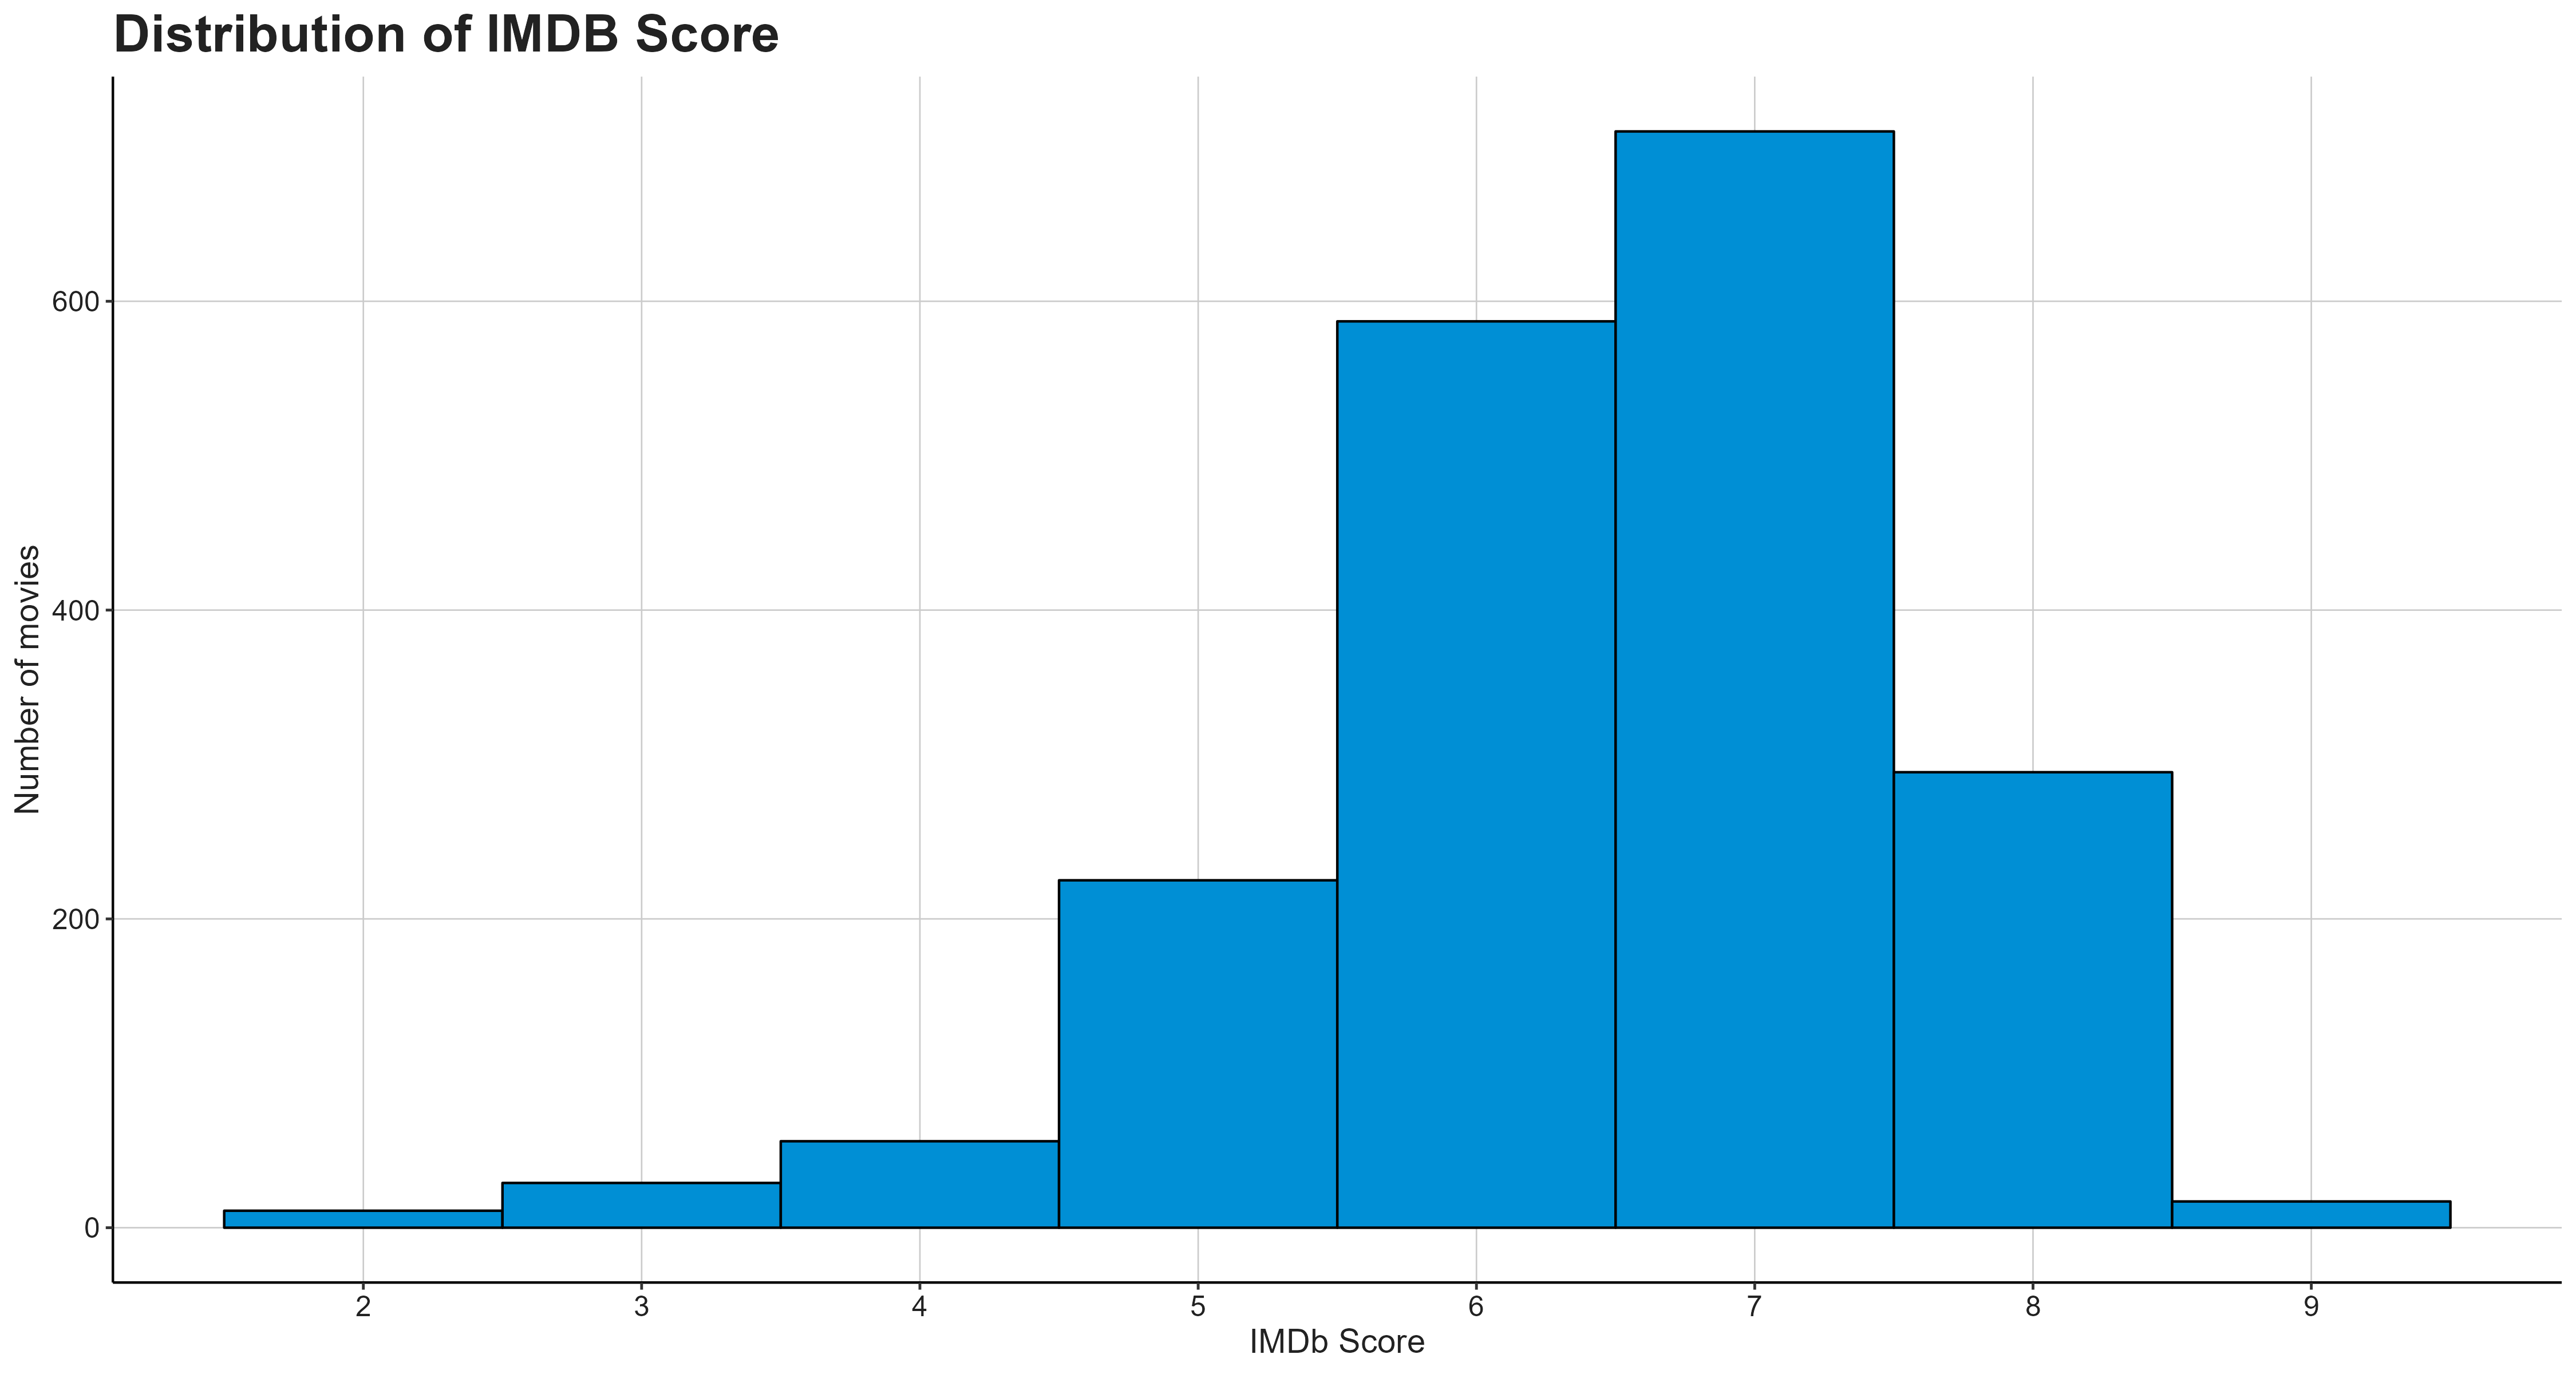
\includegraphics[width=0.75\textwidth]{imdb_score.png}
        \caption{Distribution of IMDb score}
        \label{fig:imdb-score-hist}
    \end{figure}

    \begin{figure}[h]
        \begin{subfigure}[t]{0.5\textwidth}
            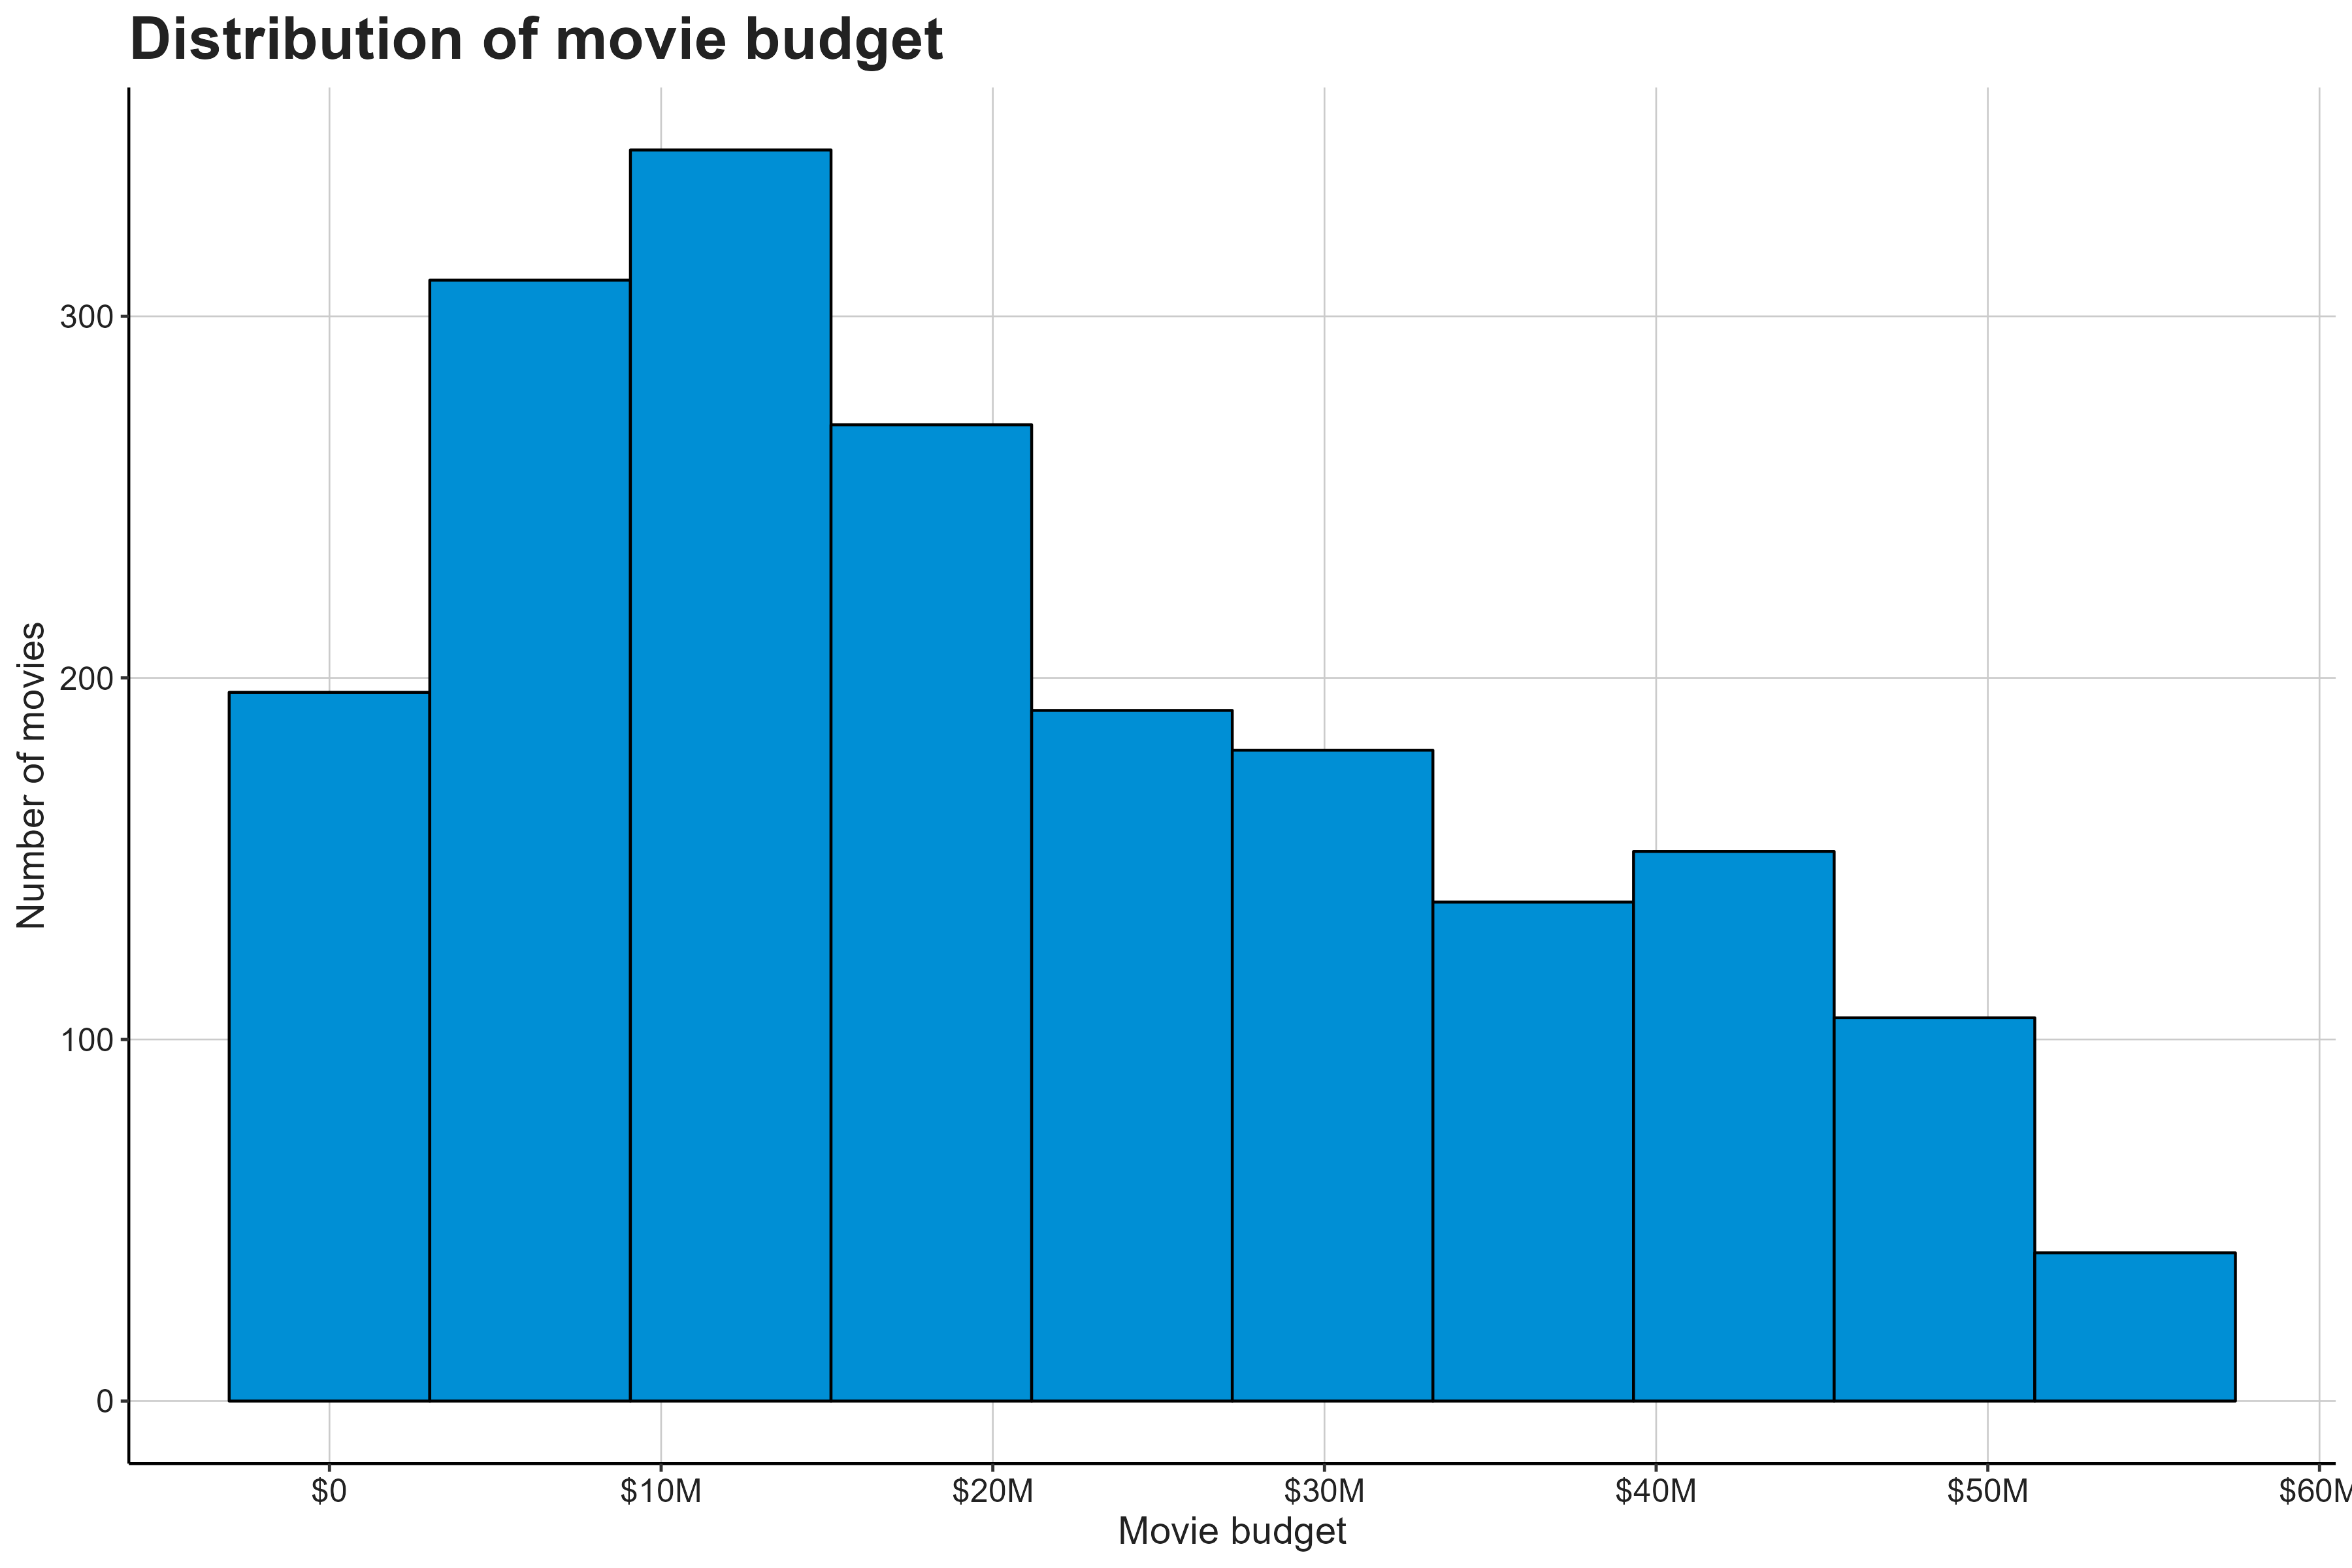
\includegraphics[width=0.95\linewidth, height=6cm]{movie_budget.png}
            \caption{Distribution of movie budget}
            \label{fig:budget-hist}
        \end{subfigure}
        ~
        \begin{subfigure}[t]{0.5\textwidth}
            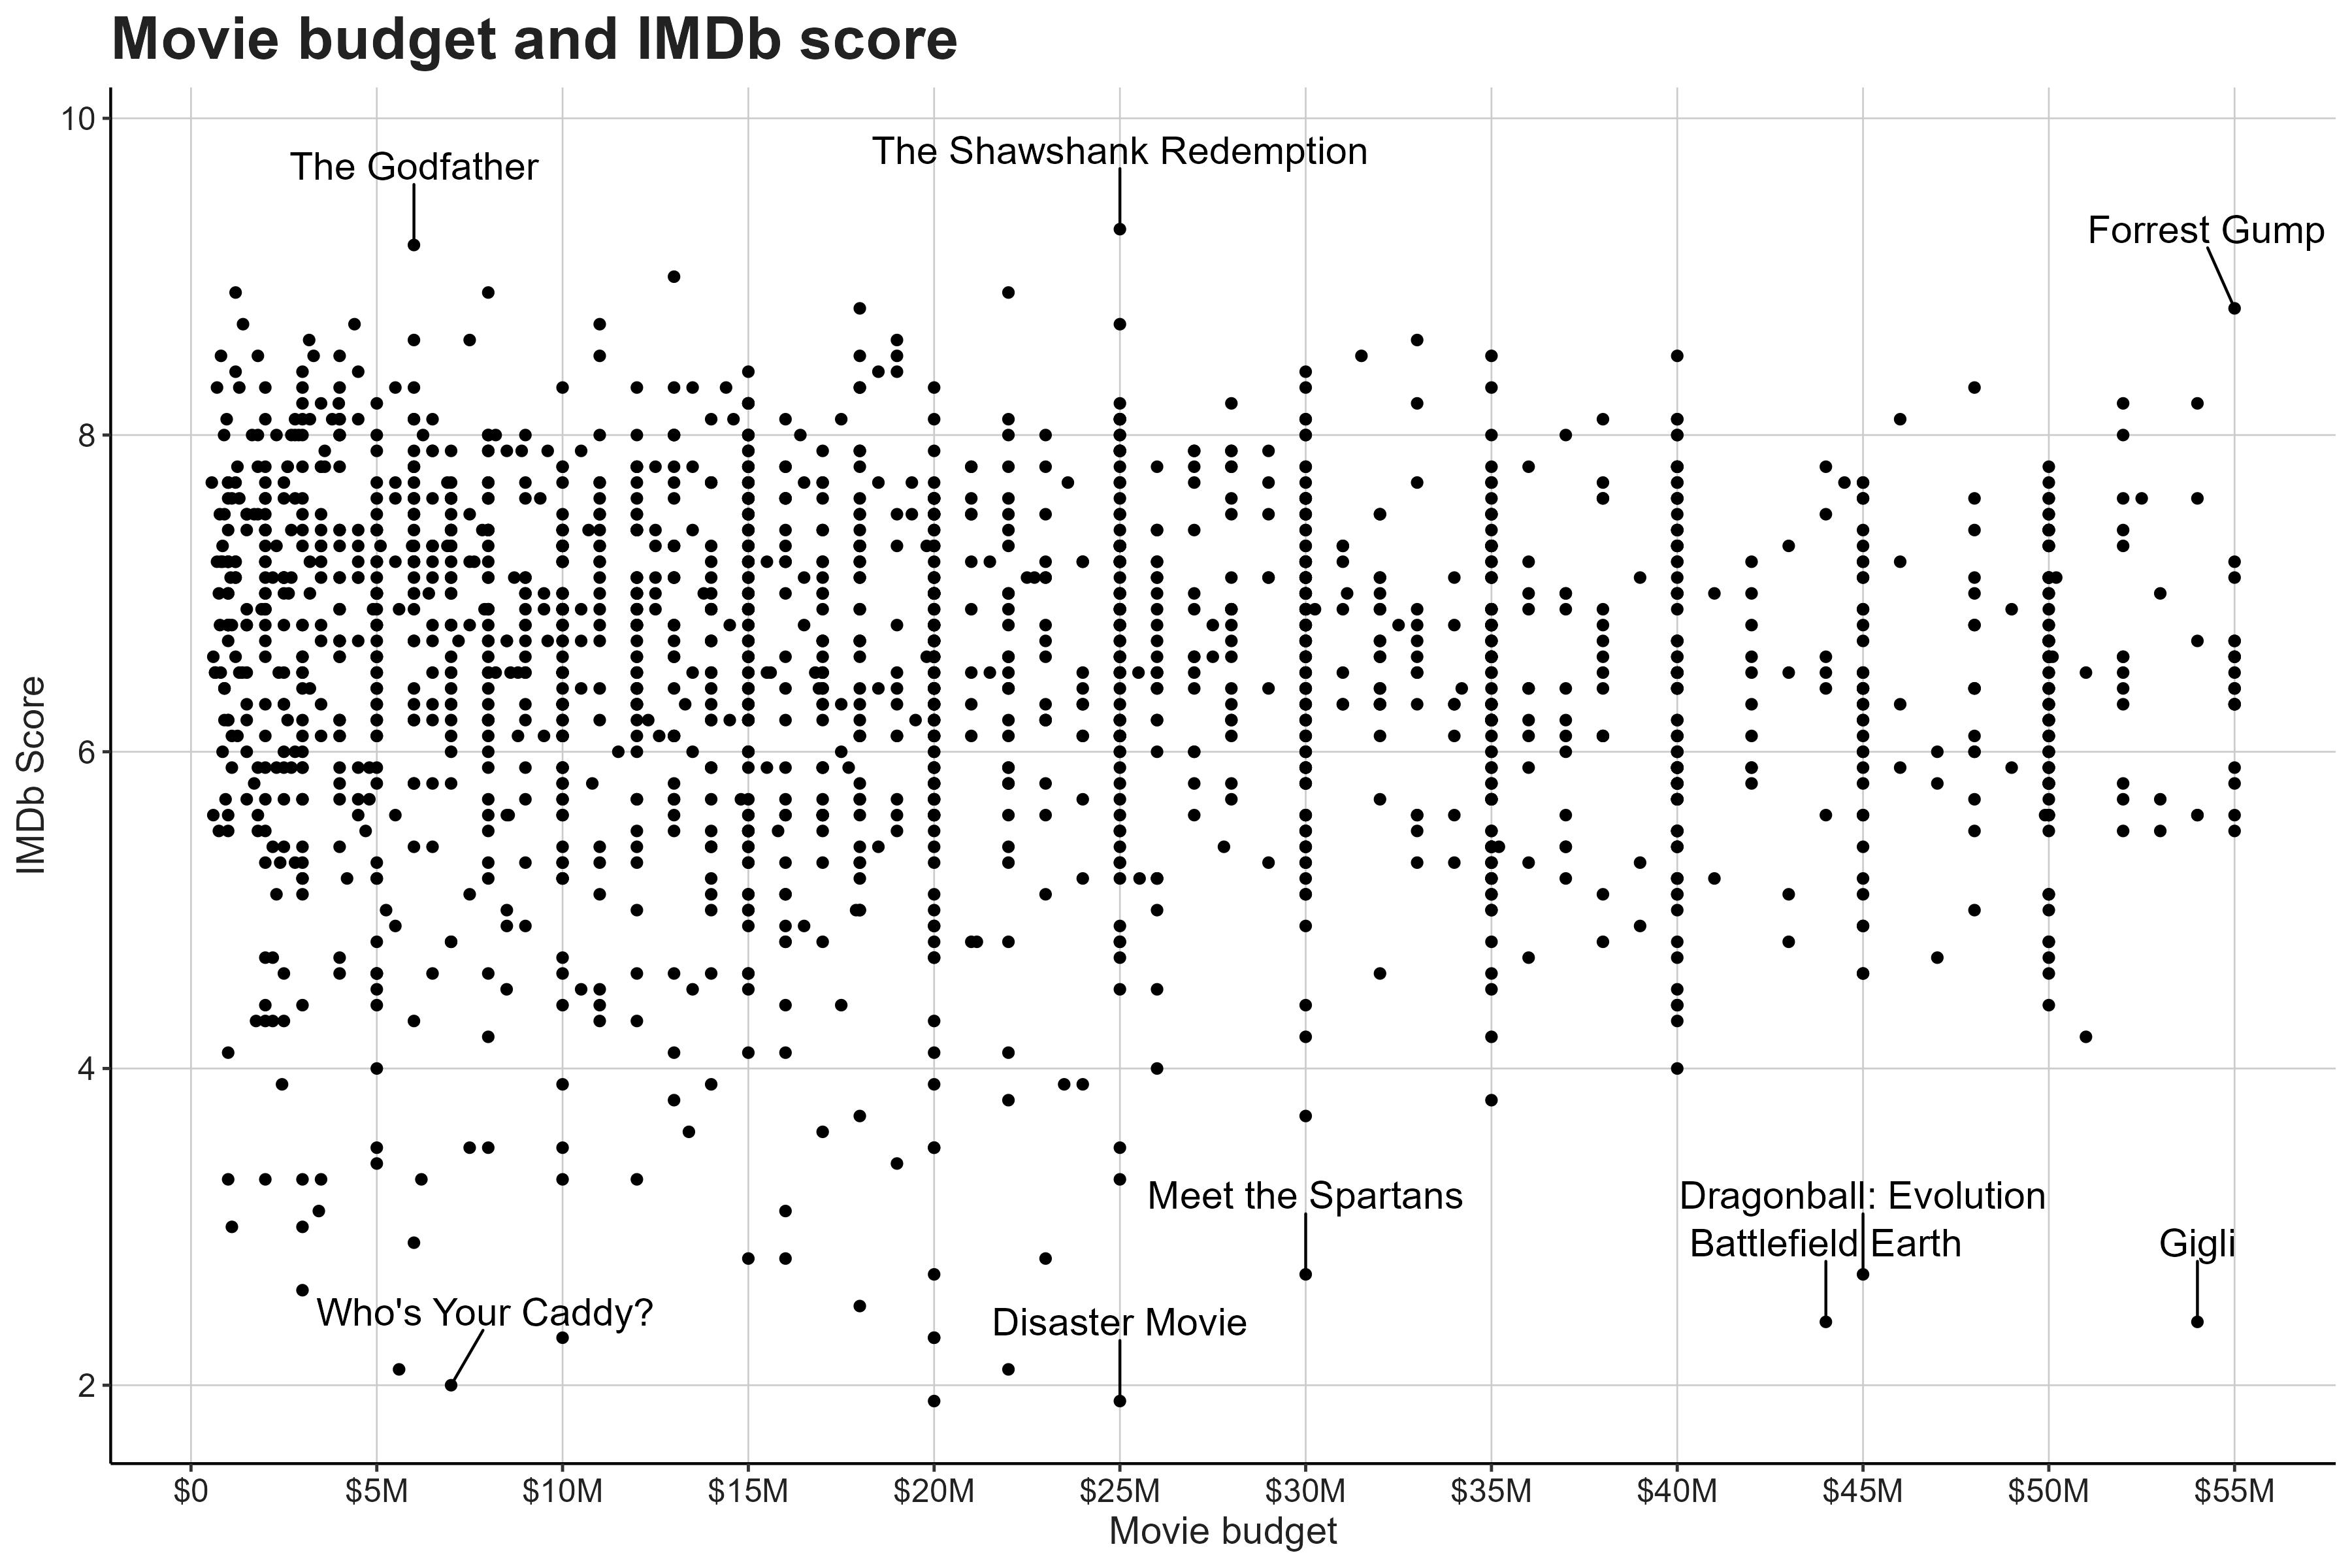
\includegraphics[width=0.95\linewidth, height=6cm]{movie_budget_imdb_score.png}
            \caption{IMDb score vs. movie budget}
            \label{fig:budget-imdb-scatter}
        \end{subfigure}

        \caption{Movie budget}
        \label{fig:budget}
    \end{figure}

    \begin{figure}[h]
        \begin{subfigure}[t]{0.5\textwidth}
            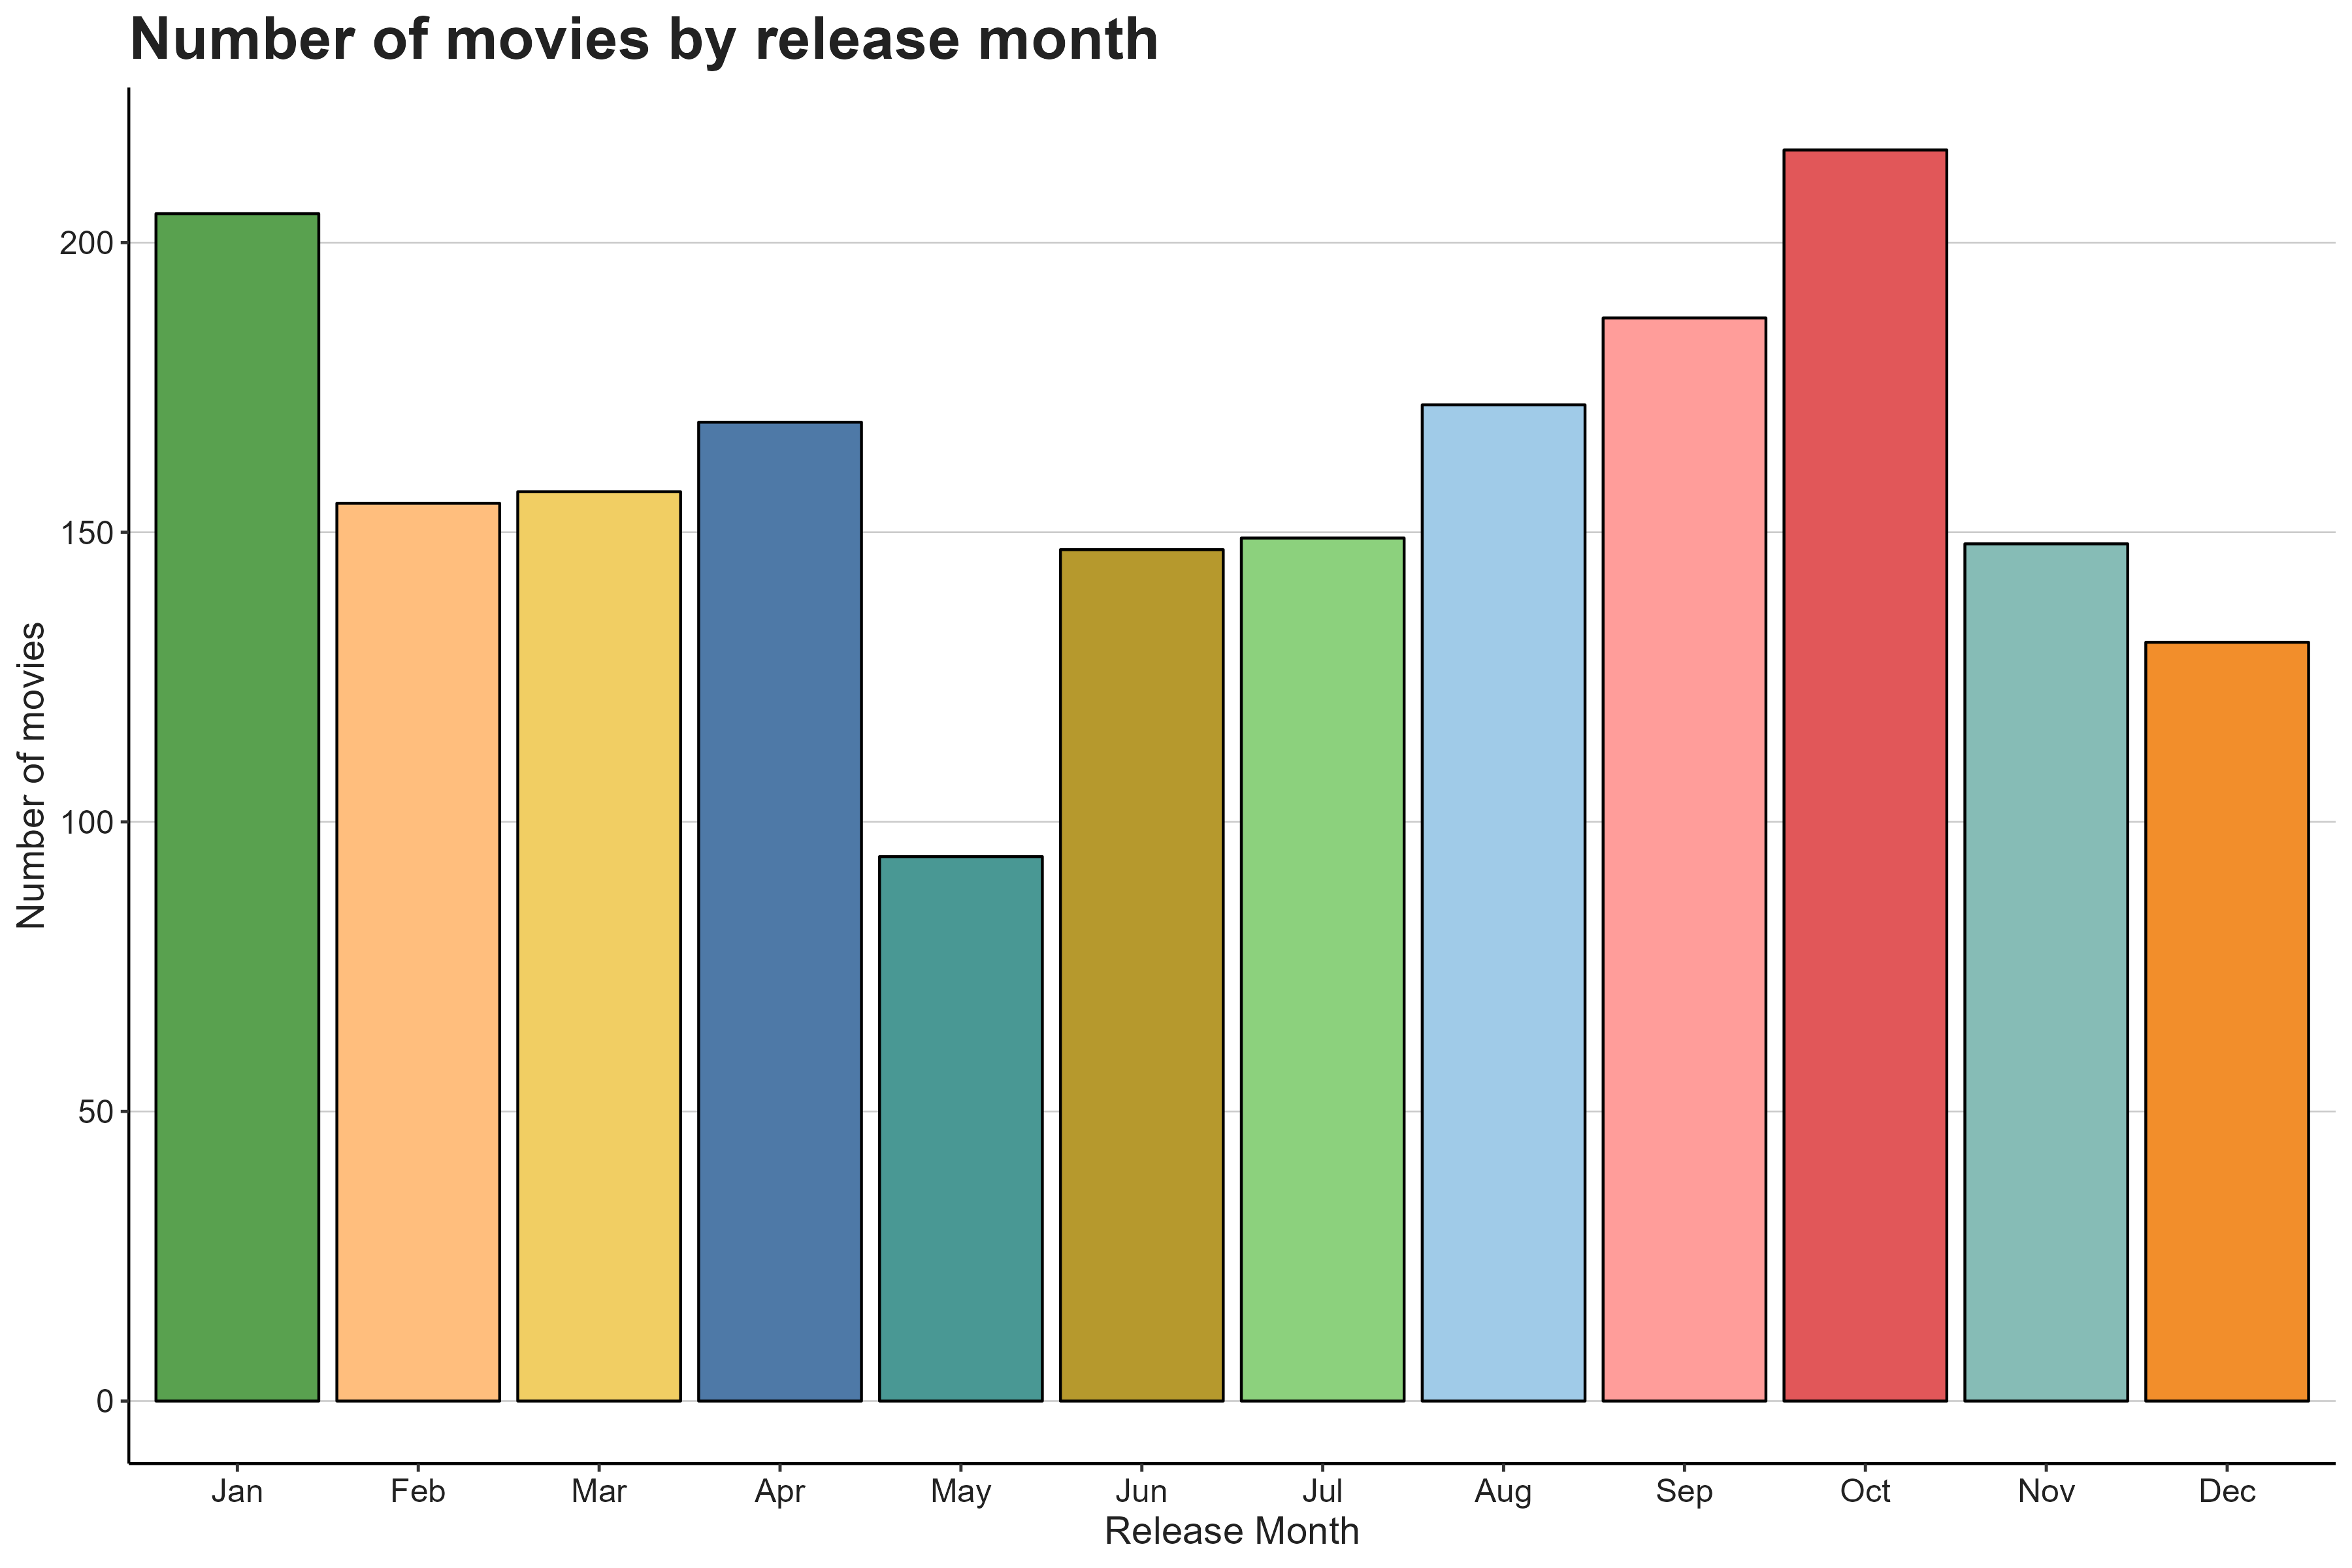
\includegraphics[width=0.95\linewidth, height=6cm]{release_month.png}
            \caption{Number of movies by release month}
            \label{fig:release-month-bar}
        \end{subfigure}
        ~
        \begin{subfigure}[t]{0.5\textwidth}
            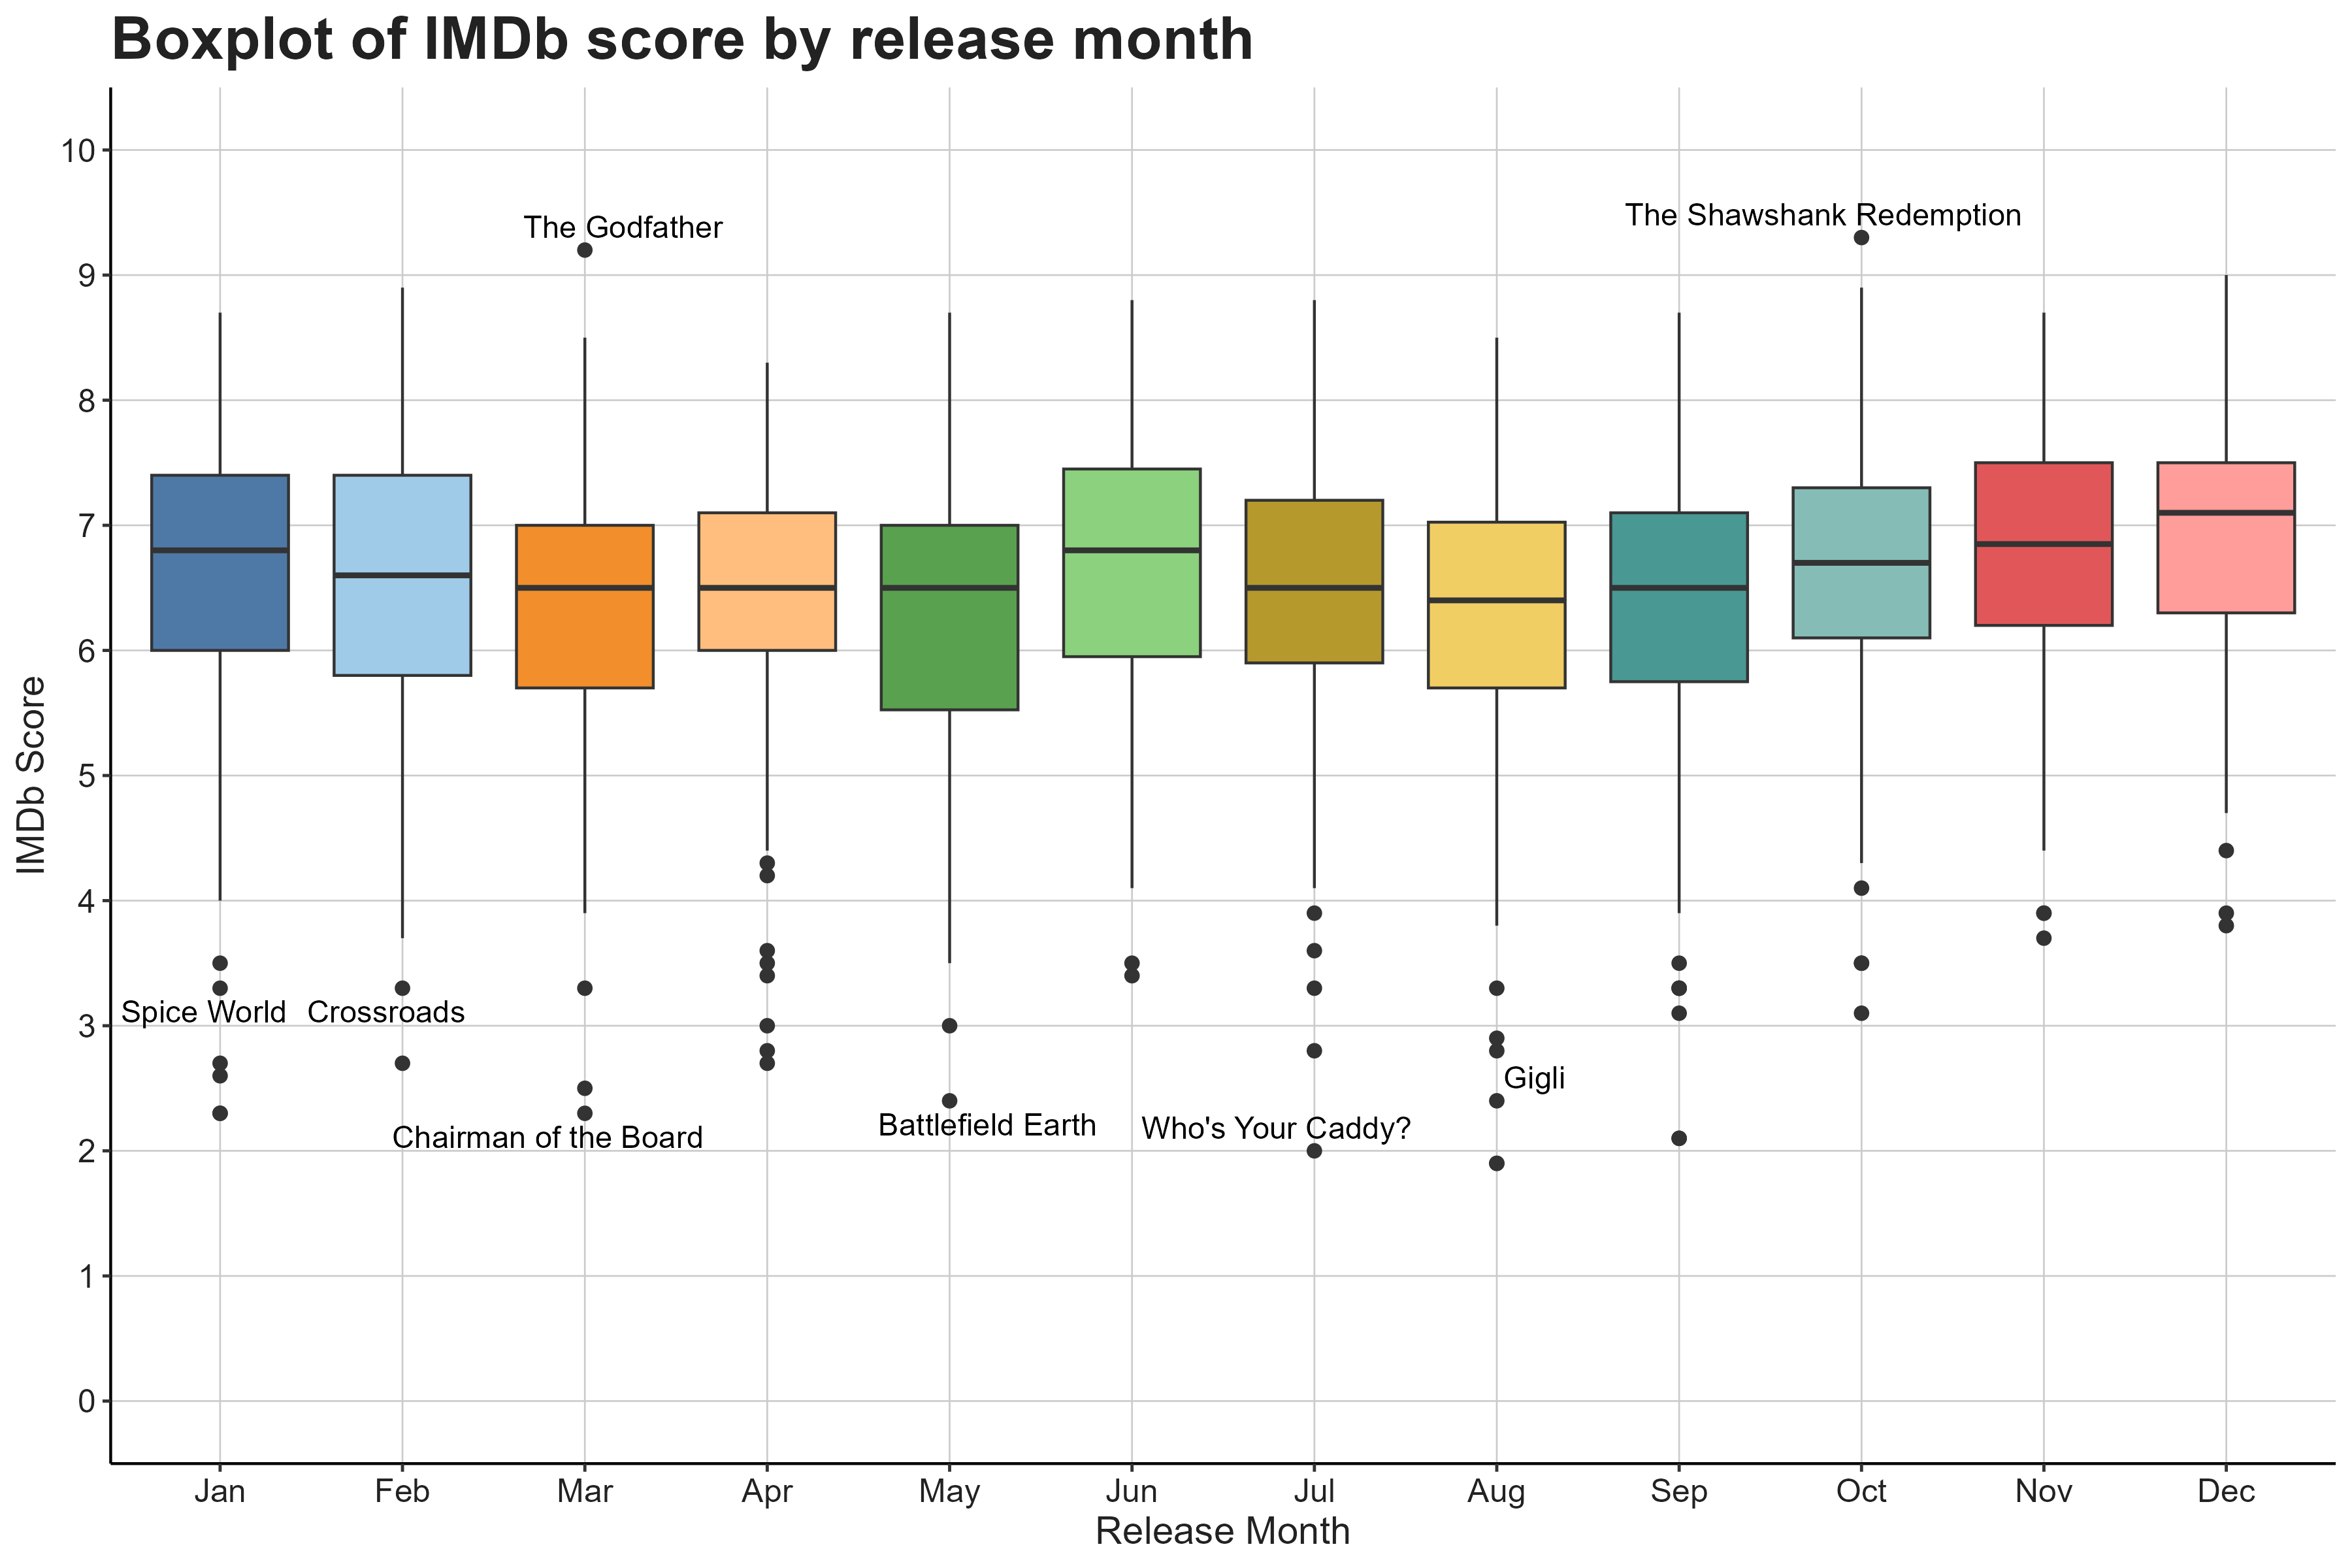
\includegraphics[width=0.95\linewidth, height=6cm]{release_month_imdb_score.png}
            \caption{IMDb score vs. release month}
            \label{fig:release-month-box}
        \end{subfigure}

        \caption{Release month}
        \label{fig:release-month}
    \end{figure}

    \begin{figure}[h]
        \centering
        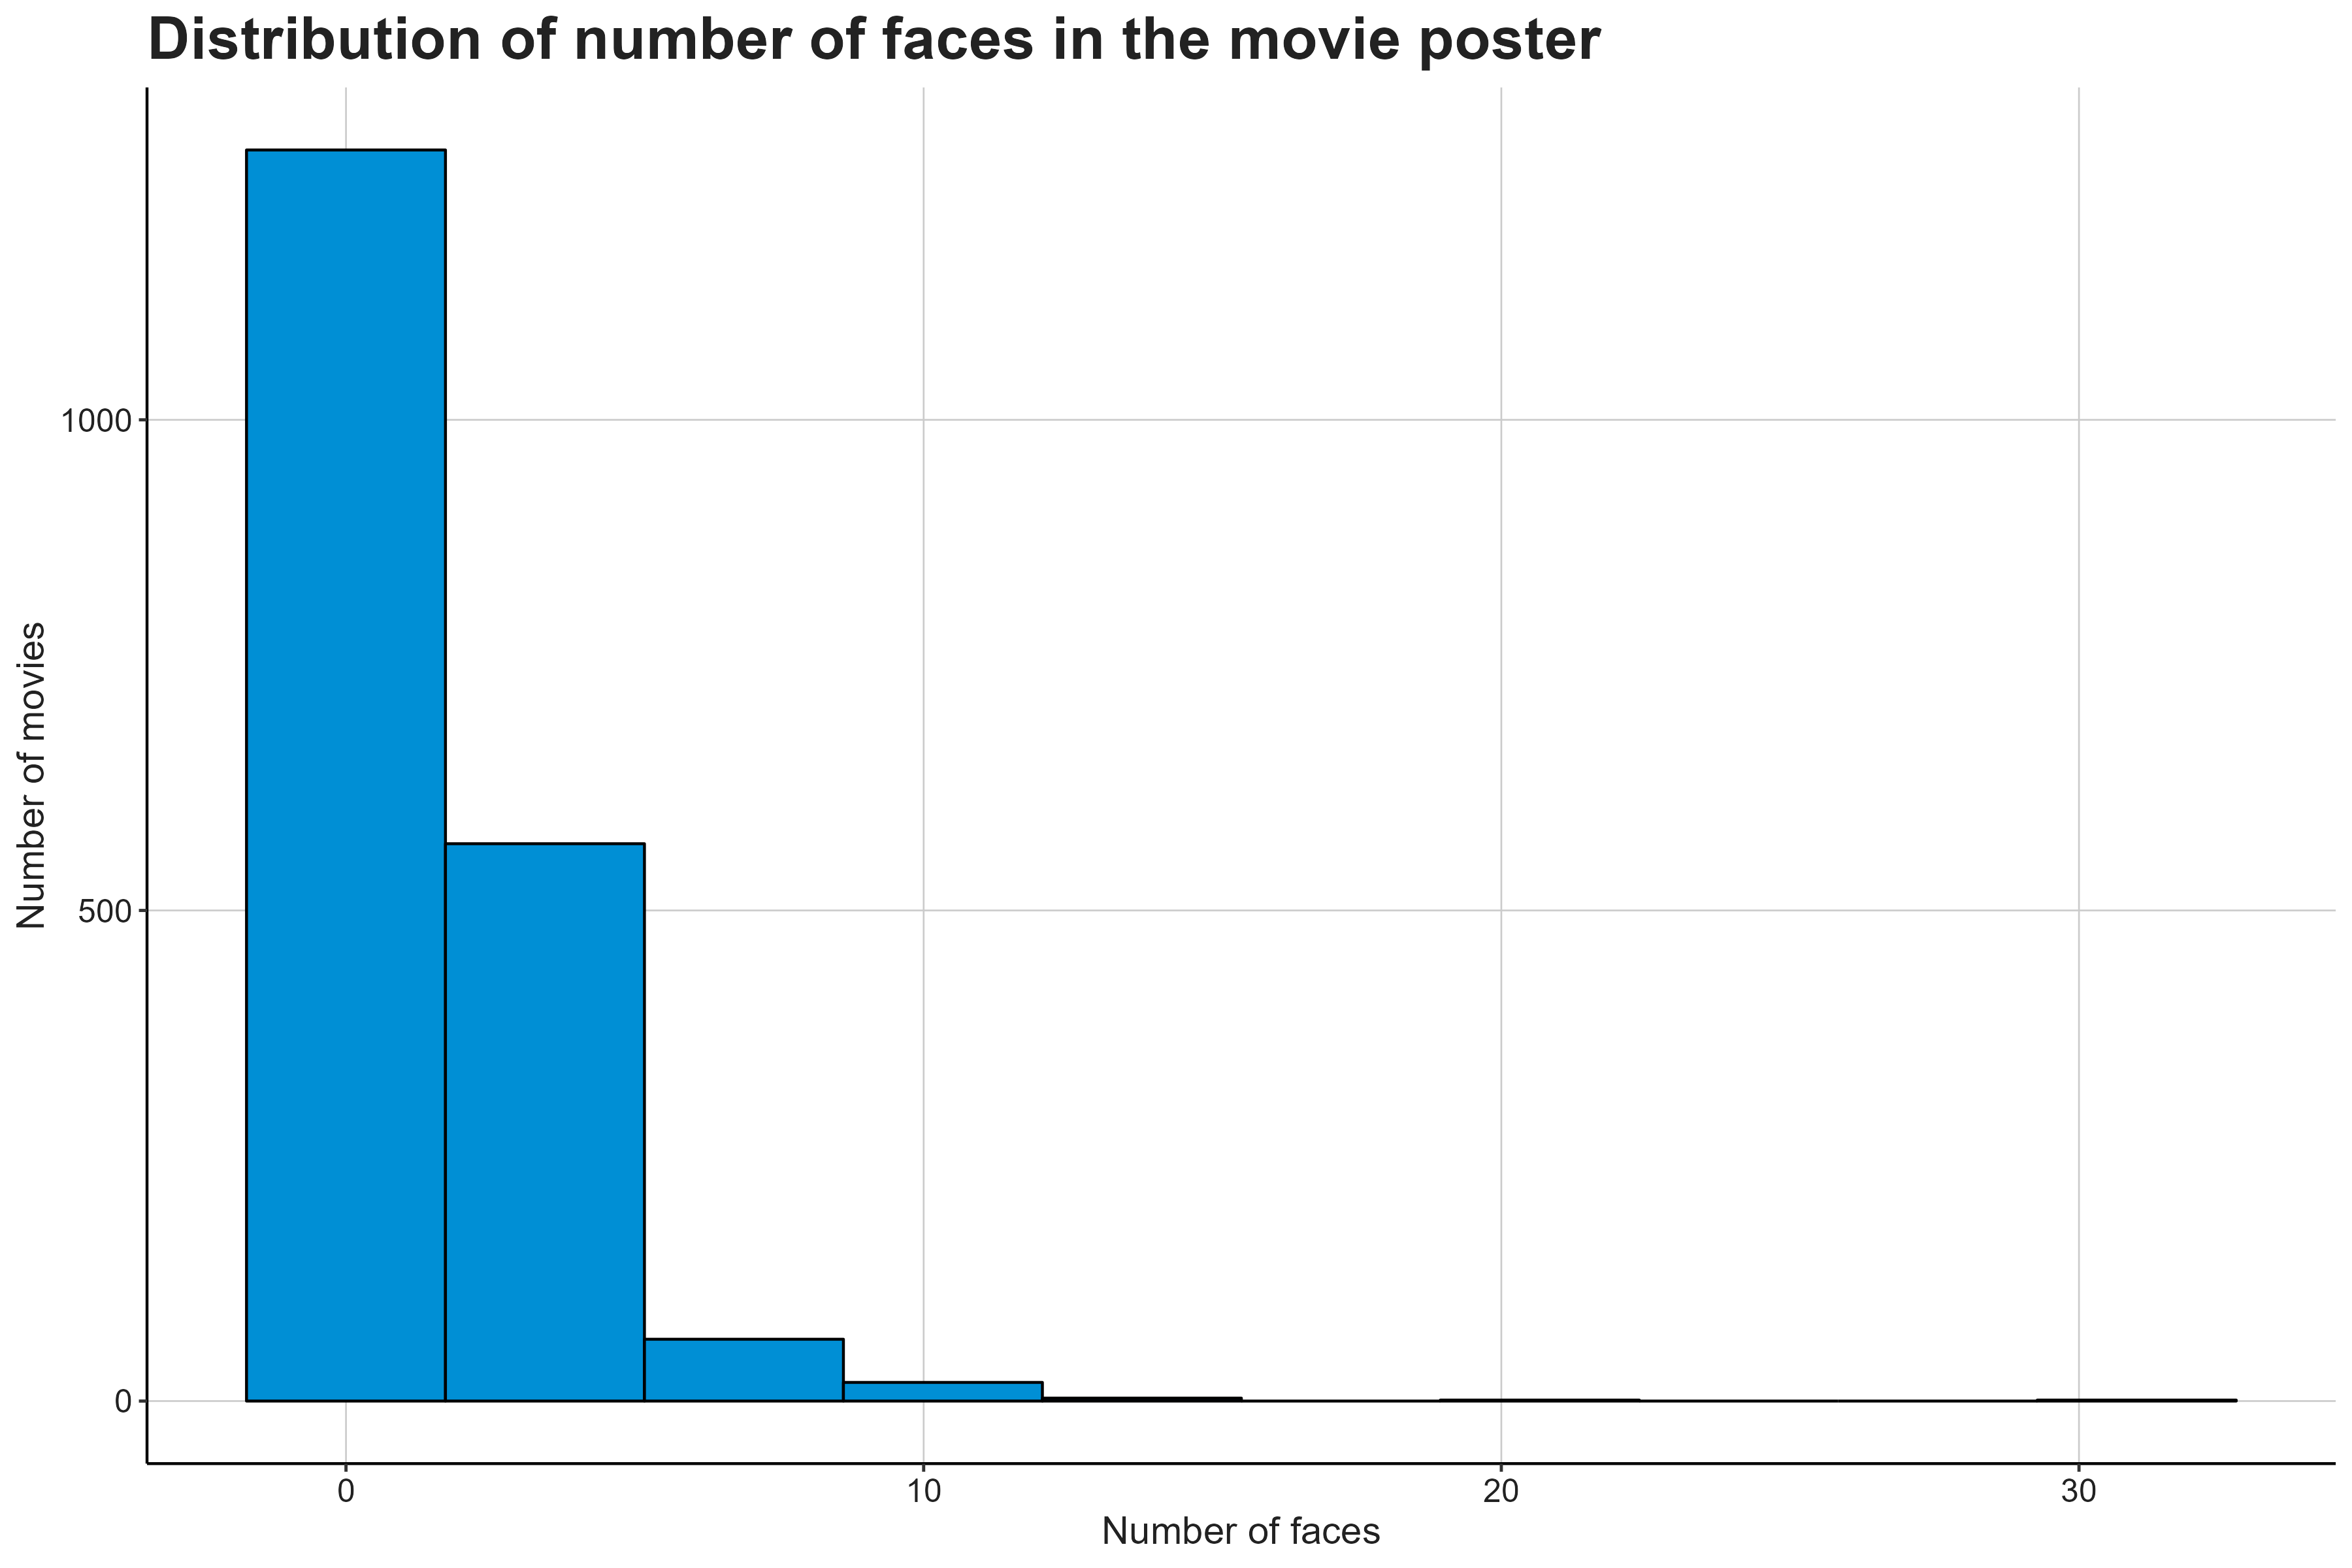
\includegraphics[width=0.75\textwidth]{number_faces.png}
        \caption{Distribution of number of faces}
        \label{fig:faces-hist}
    \end{figure}

    \begin{figure}[h]

        \begin{subfigure}[t]{0.5\textwidth}
            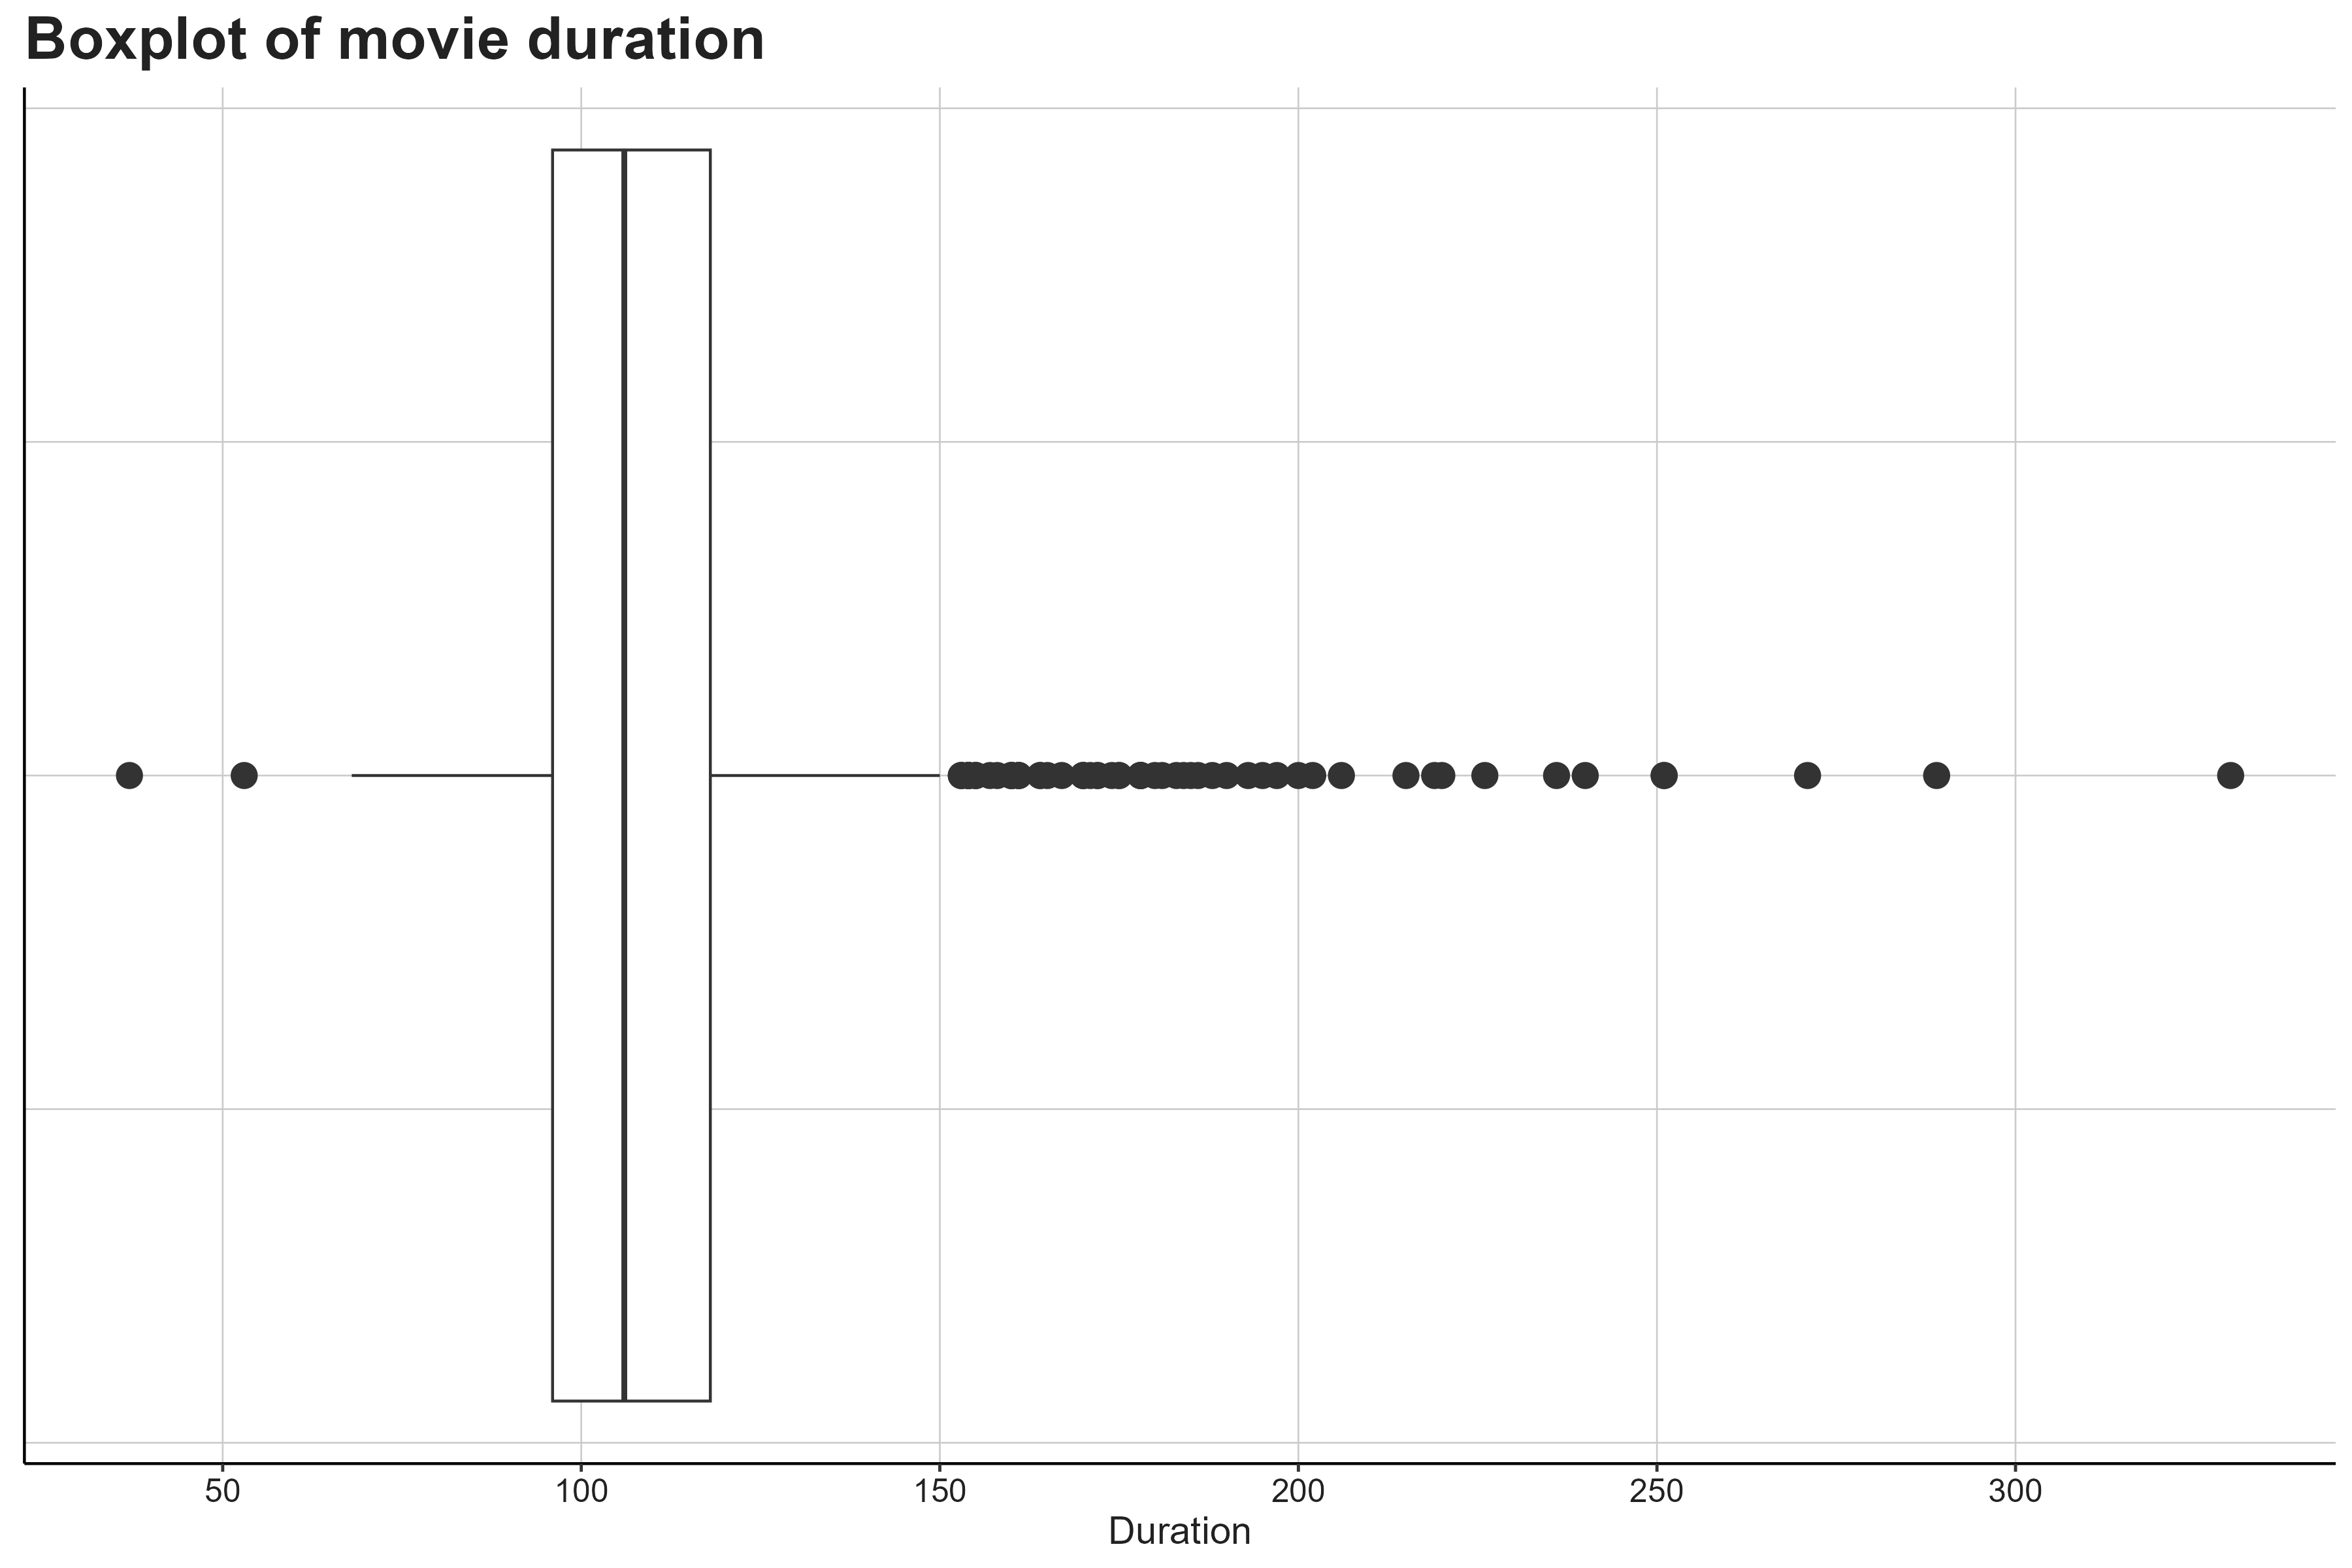
\includegraphics[width=0.95\linewidth]{duration.png}
            \caption{Boxplot of duration}
            \label{fig:duration-boxplot}
        \end{subfigure}
        ~
        \begin{subfigure}[t]{0.5\textwidth}
            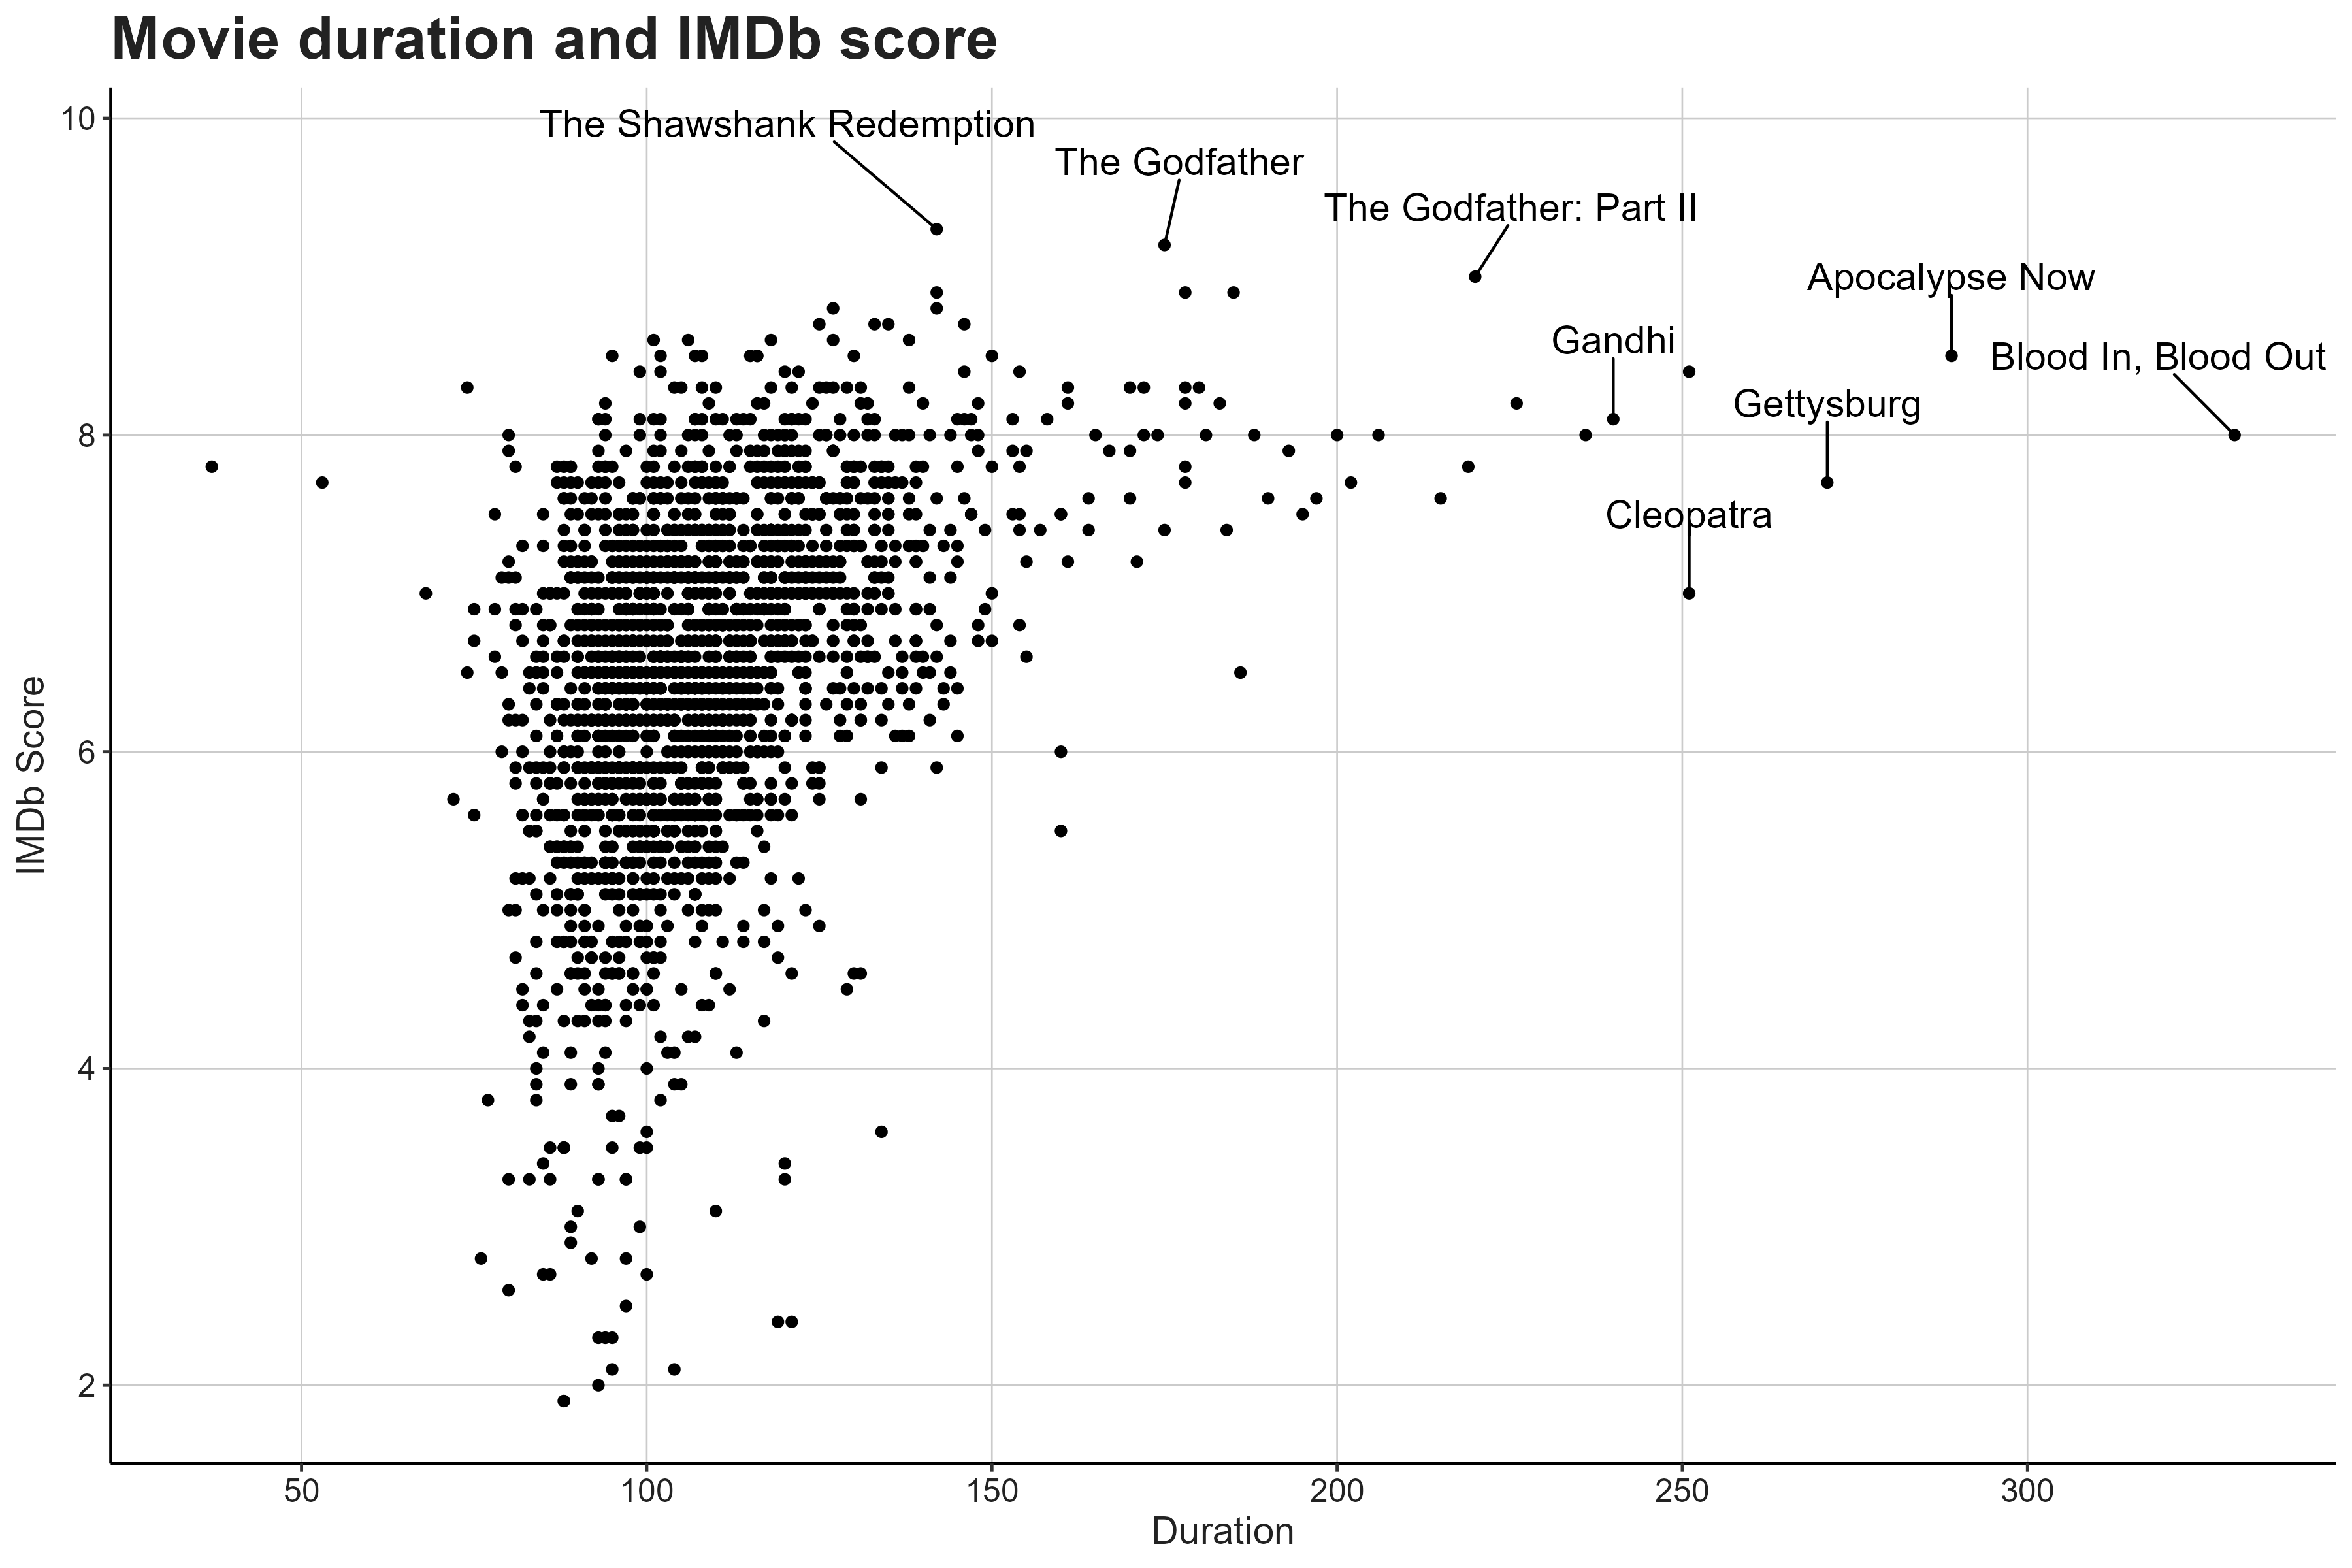
\includegraphics[width=0.95\linewidth]{duration_imdb_score.png}
            \caption{IMDb score vs. duration}
            \label{fig:duration-scatter}
        \end{subfigure}

        \caption{Duration}
        \label{fig:duration}
    \end{figure}

    \begin{figure}[h]
        \centering
        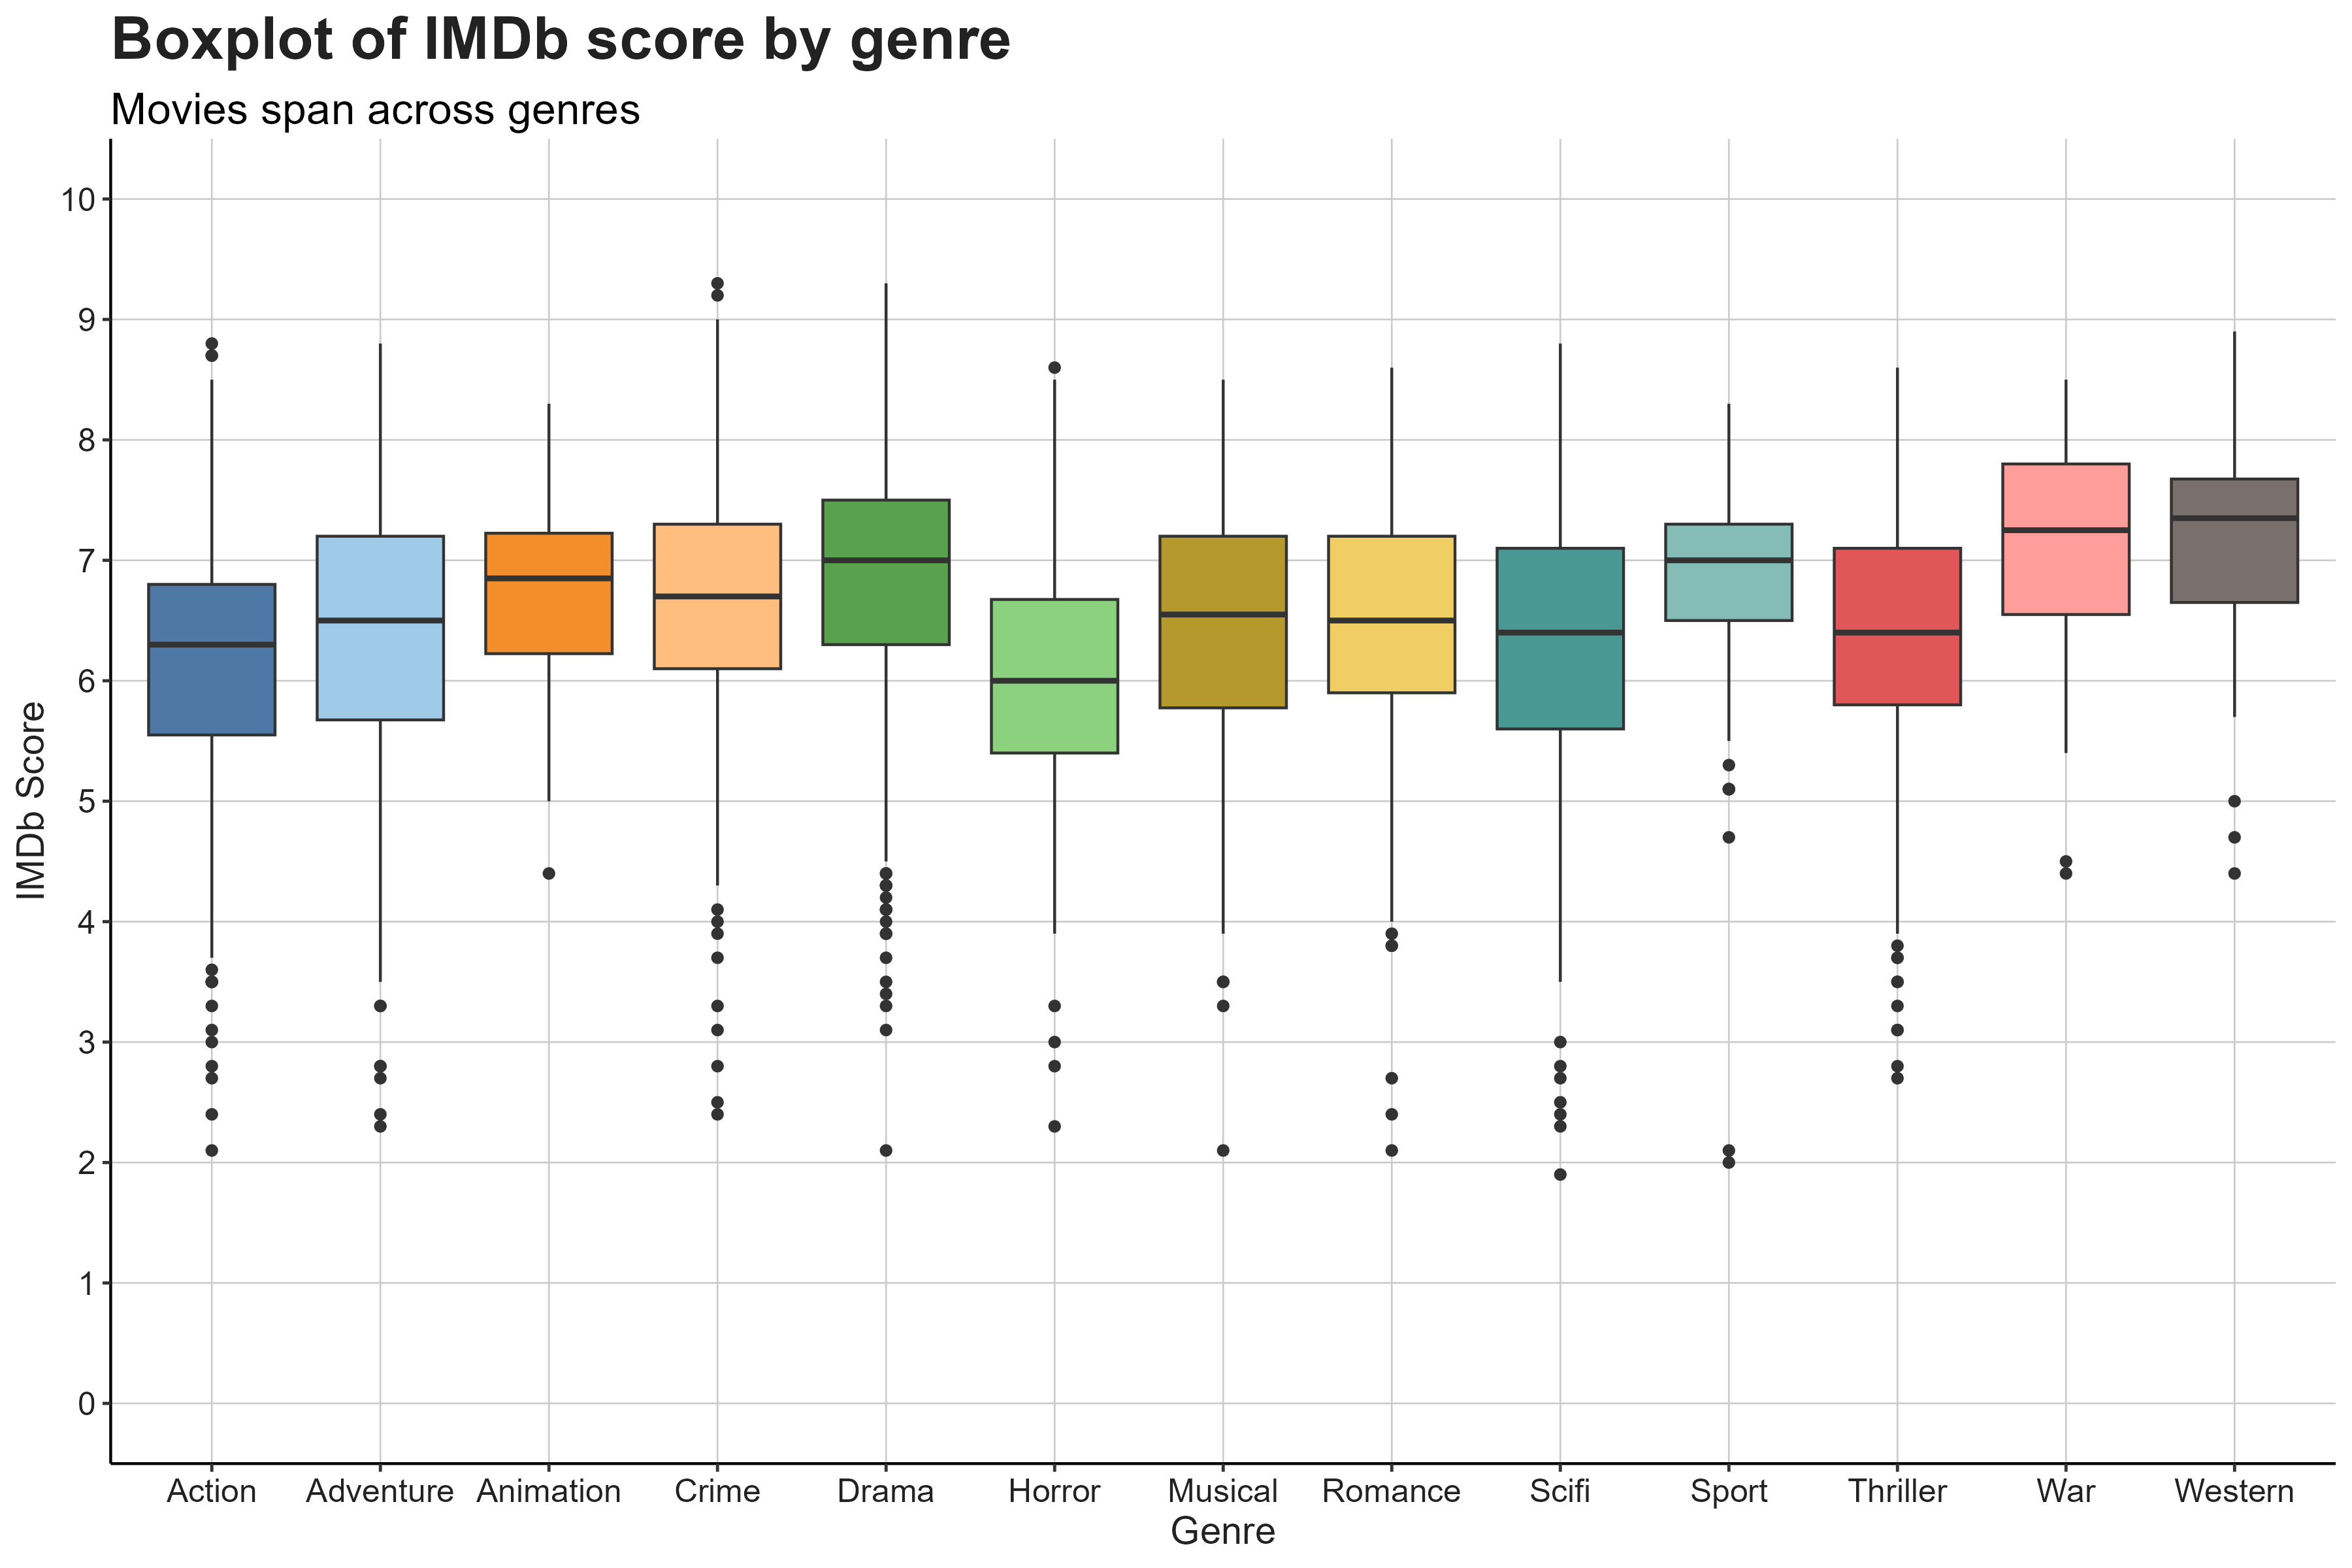
\includegraphics[width=0.75\textwidth]{genre_imdb_score.png}
        \caption{Distribution of ratings across genres}
        \label{fig:genre-bar}
    \end{figure}

    \begin{figure}[h]
        \centering
        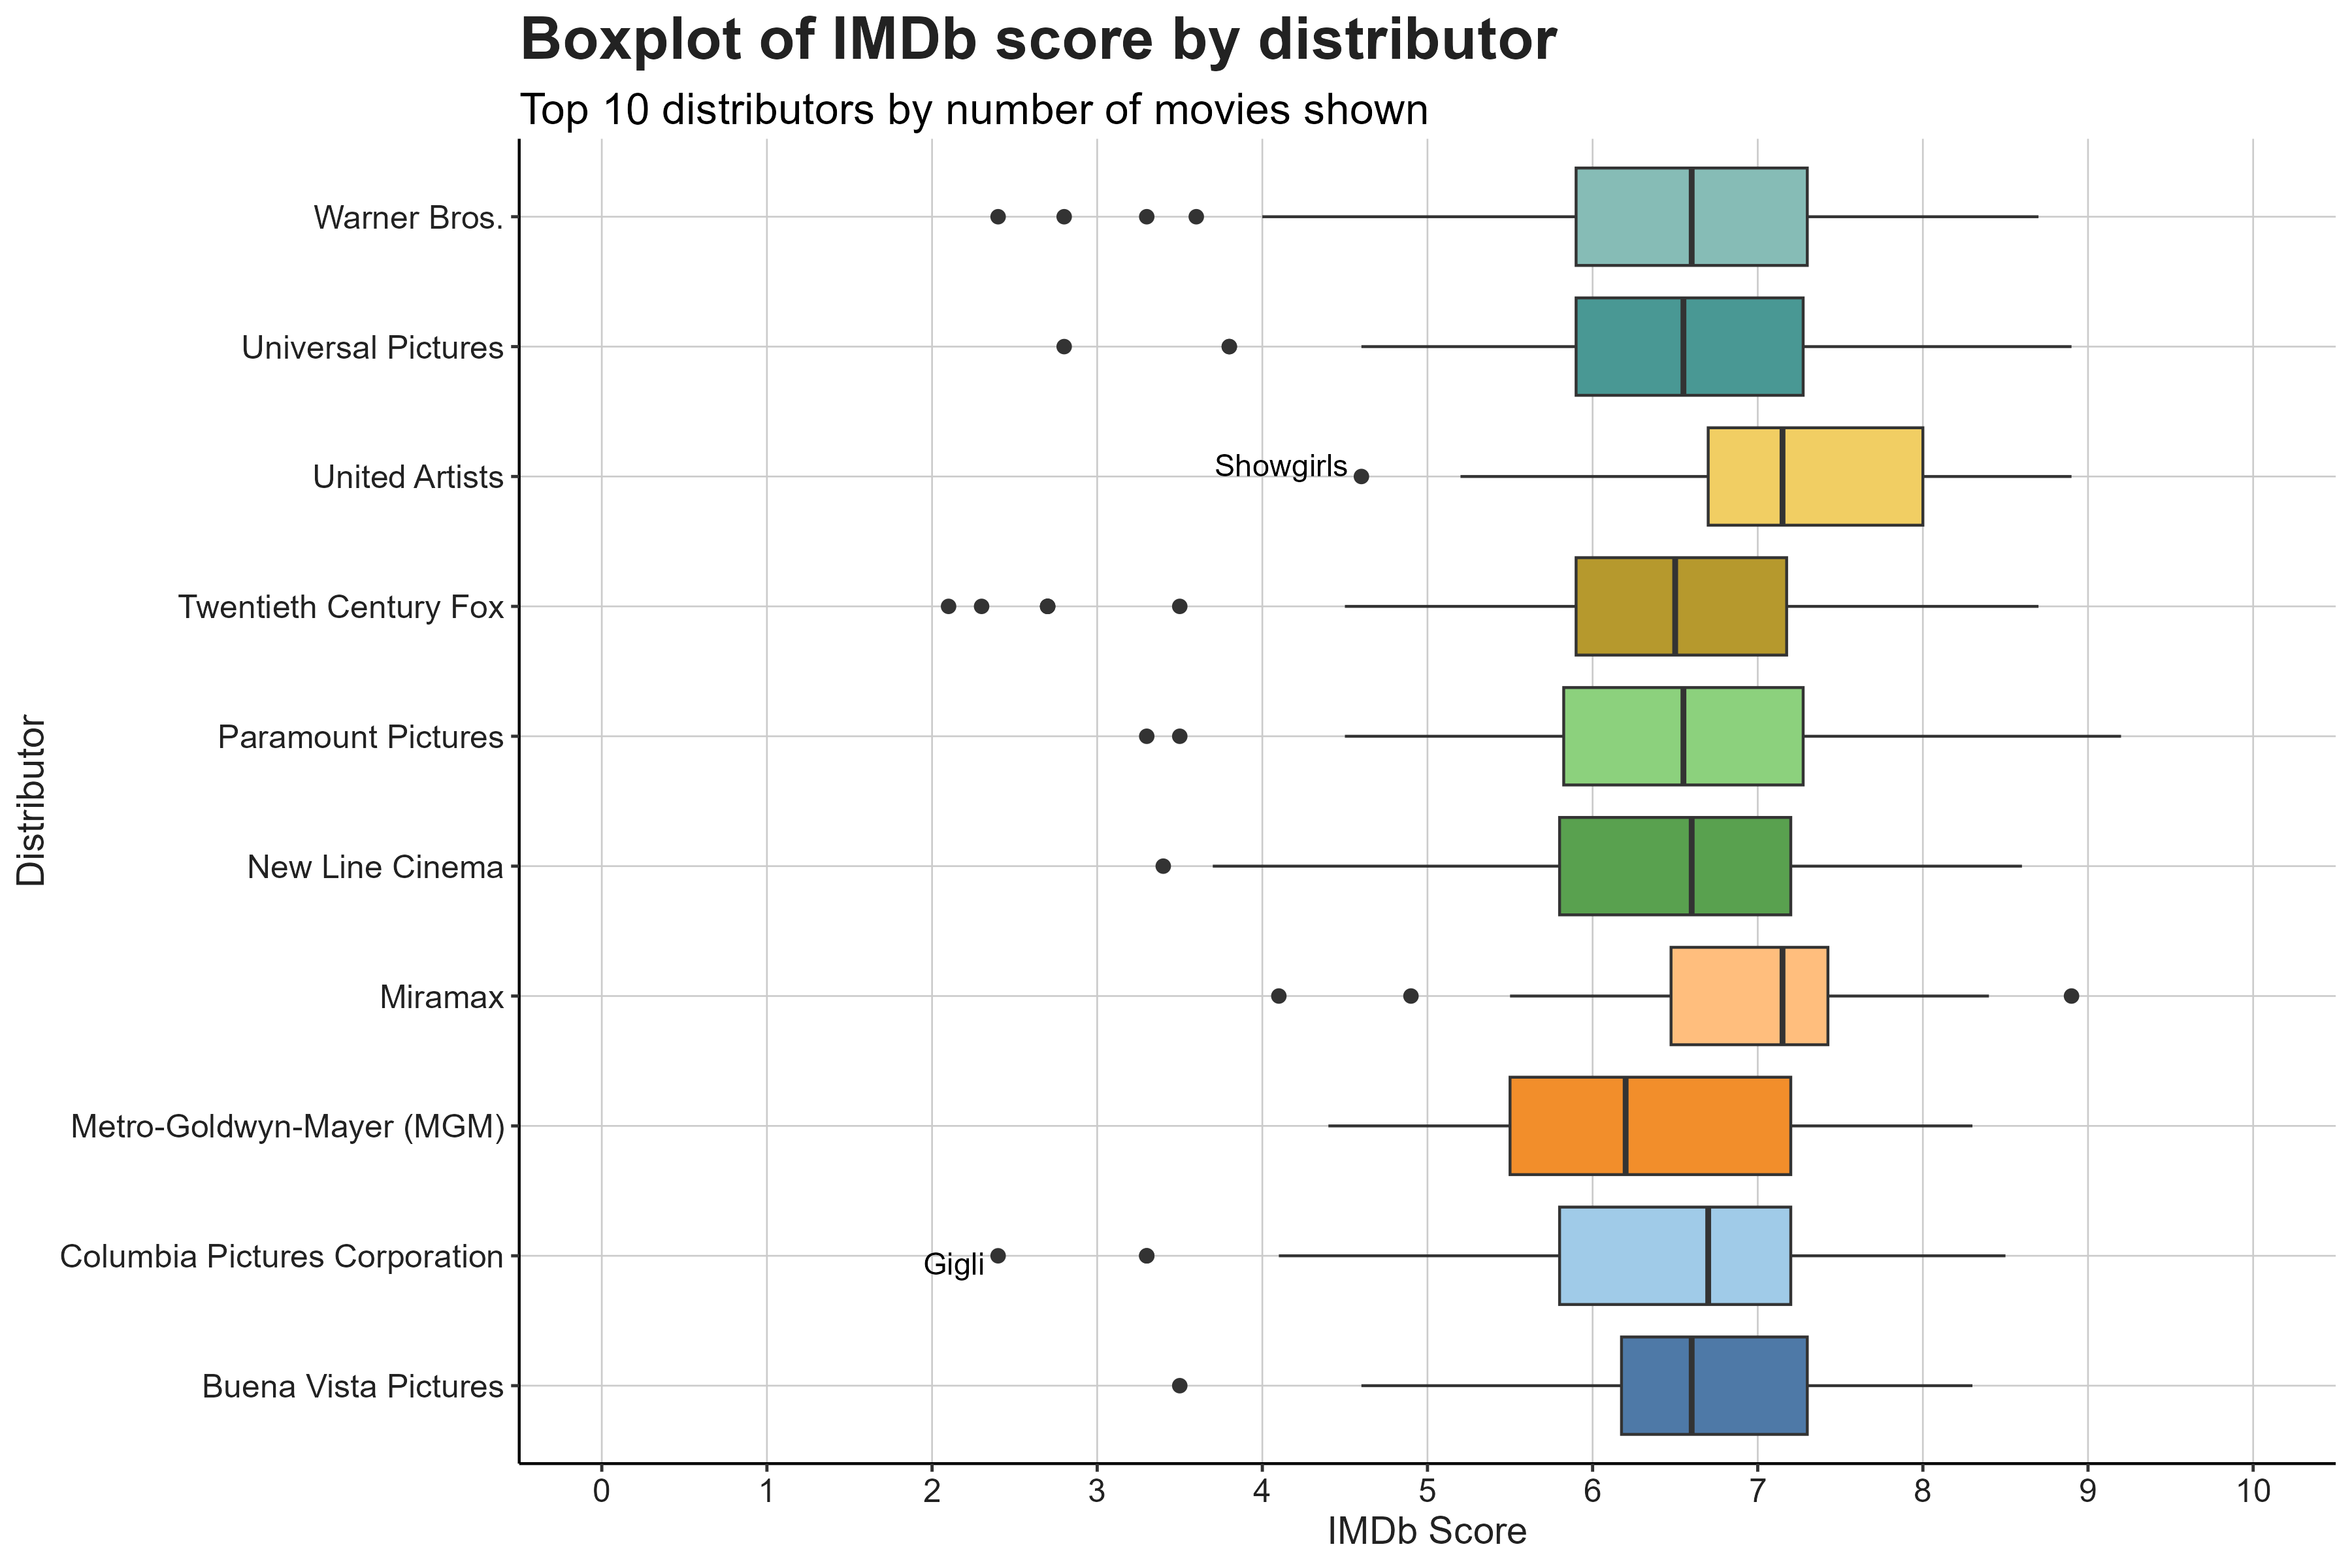
\includegraphics[width=0.75\textwidth]{distributor_imdb_score.png}
        \caption{Distribution of movies across distributors}
        \label{fig:distributor-bar}
    \end{figure}

    \begin{figure}[h]
        \centering
        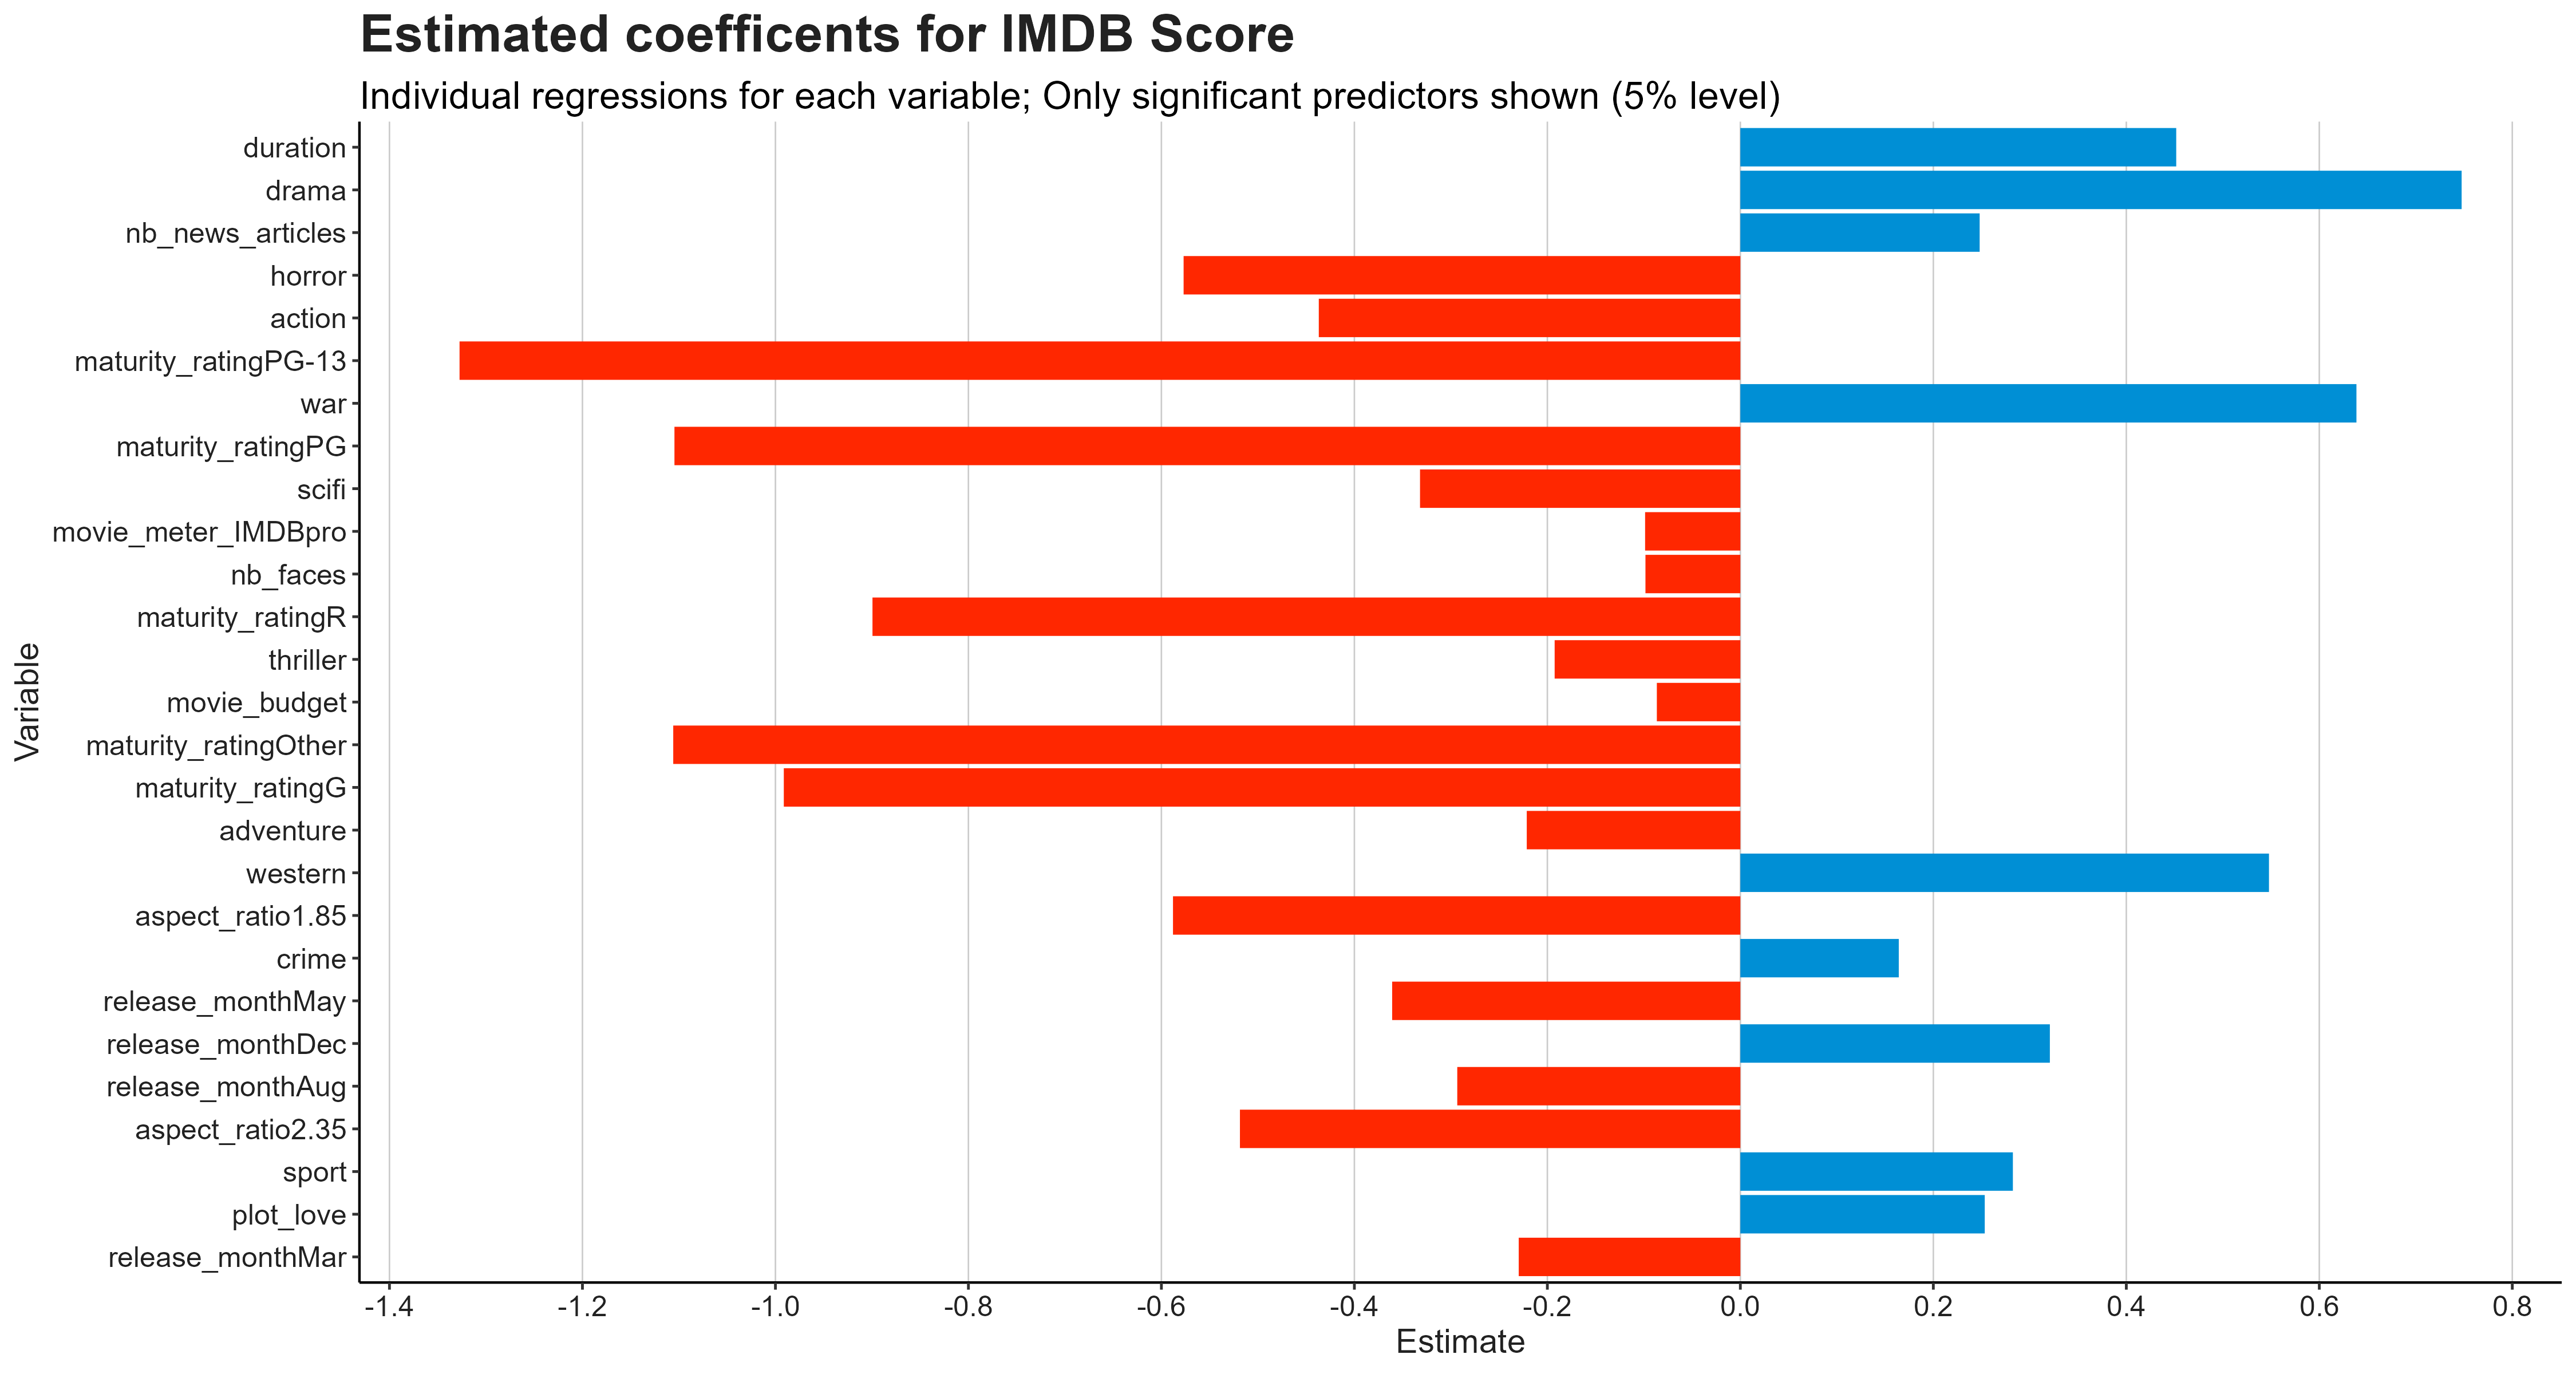
\includegraphics[width=0.75\textwidth]{individual_regressions.png}
        \caption{Individual regressions}
        \label{fig:individual-coefficients}
    \end{figure}

    \begin{figure}[h]
        \centering
        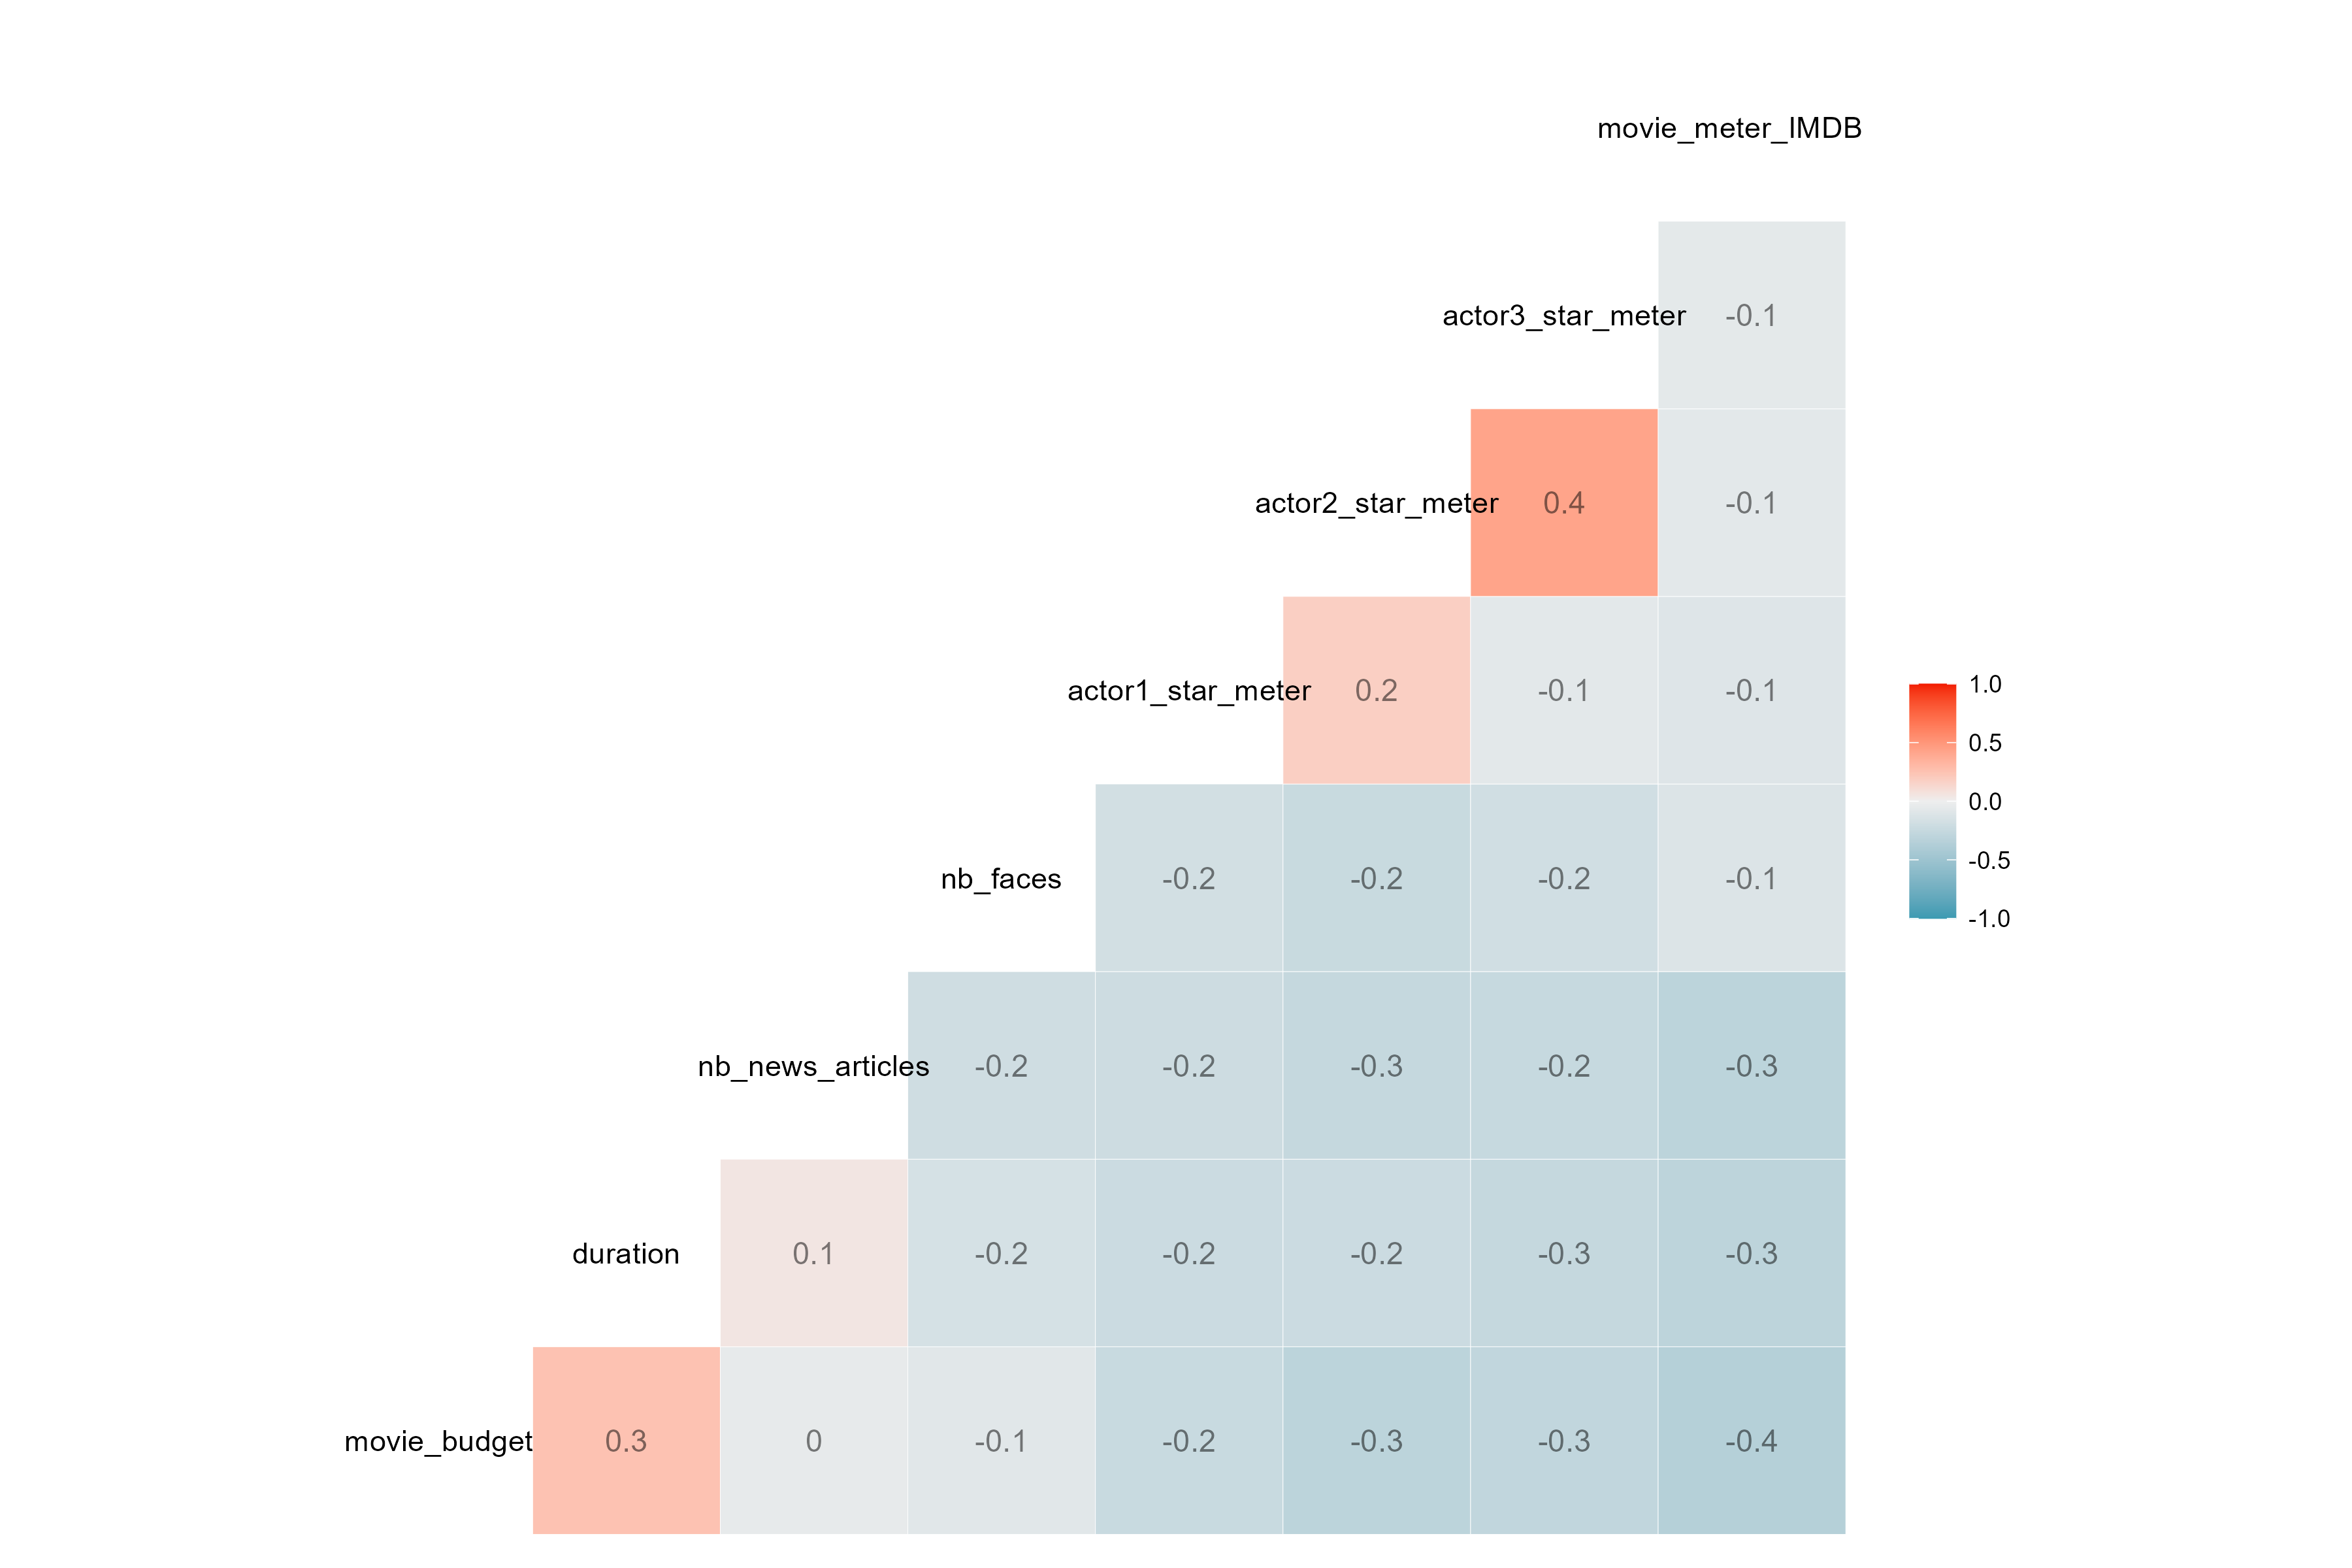
\includegraphics[width=0.75\textwidth]{corr_plot.png}
        \caption{Correlation matrix}
        \label{fig:correlation-matrix}
    \end{figure}

    \clearpage
    \section{Tables}\label{app:tables}

    \begin{table}[h]
        \centering
        \begin{tabular}{|l|l|}
            \hline
            \textbf{Numerical Predictors}    & \textbf{Categorical Predictors} \\
            \hline
            \texttt{Movie Budget}            & \texttt{Release month}          \\
            \texttt{Duration}                & \texttt{Maturity rating}        \\
            \texttt{Number of faces}         & \texttt{Aspect ratio}           \\
            \texttt{Number of news articles} & \texttt{Genre}                  \\
            \texttt{Movie meter IMDBPro}     & \texttt{Plot keywords}          \\
            \hline
        \end{tabular}
        \caption{List of Predictors}
        \label{tab:predictors}
    \end{table}

    \begin{table}[h]
        \centering
        \begin{tabular}{|l|l|l|l|}
            \hline
            \textbf{Metric}      & \textbf{Linear} & \textbf{Polynomial} & \textbf{Spline} \\
            \hline
            MSE                  & $0.76$          & $0.68$              & $0.67$          \\
            RMSE                 & $0.87$          & $0.83$              & $0.82$          \\
            $R^{2}$              & $0.38$          & $0.45$              & $0.46$          \\
            Number of predictors & $52$            & $60$                & $61$            \\
            \hline
        \end{tabular}
        \caption{Model performance ($k=20$)}
        \label{tab:model-performance}
    \end{table}

    \begin{table}[h]
        \centering
        \begin{tabular}{|l|p{6cm}|l|l|l|l|}
            \hline
            \textbf{Row ID} & \textbf{Movie Title}                                 & \textbf{Release Date} & \textbf{Linear} & \textbf{Polynomial} & \textbf{Spline} \\
            \hline
            1               & Pencils vs Pixels                                    & 2023-11-07            & $6.19$          & $5.87$              & $3.44$          \\
            2               & The Dirty South                                      & 2023-11-10            & $6.45$          & $5.41$              & $3.40$          \\
            3               & The Marvels                                          & 2023-11-10            & $6.82$          & $7.08$              & $9.41$          \\
            4               & The Holdovers                                        & 2023-11-10            & $7.22$          & $7.66$              & $8.70$          \\
            5               & Next Goal Wins                                       & 2023-11-17            & $6.78$          & $7.43$              & $8.59$          \\
            6               & Thanksgiving                                         & 2023-11-17            & $6.31$          & $7.13$              & $9.66$          \\
            7               & The Hunger Games: The Ballad of Songbirds and Snakes & 2023-11-17            & $7.02$          & $7.90$              & $10.38$         \\
            8               & Trolls Band Together                                 & 2023-11-17            & $7.01$          & $7.71$              & $8.88$          \\
            9               & Leo                                                  & 2023-11-21            & $6.92$          & $6.41$              & $5.08$          \\
            10              & Dream Scenario                                       & 2023-11-22            & $6.43$          & $7.10$              & $8.28$          \\
            11              & Wish                                                 & 2023-11-22            & $6.86$          & $7.83$              & $10.40$         \\
            12              & Napoleon                                             & 2023-11-22            & $7.57$          & $8.32$              & $10.52$         \\
            \hline
        \end{tabular}
        \caption{Model predictions}
        \label{tab:predictions}
    \end{table}

    \begin{center}
        \begin{longtable}{@{\extracolsep{5pt}}lc}
            \caption{Final model coefficients (heteroskedasticity adjusted)}
            \label{tab:final-coefficients}
            \\\hline
            \hline                                                                                                             \\
                                                        & \multicolumn{1}{c}{\textit{Dependent variable:}}                     \\
            \cline{2-2}
            \\ & imdb\_score \\
            \hline                                                                                                             \\
            \endfirsthead

            \multicolumn{2}{c}{Table \thetable: Final model coefficients (heteroskedasticity adjusted) (Continued)}            \\
            \hline\hline                                                                                                       \\
                                                        & \multicolumn{1}{c}{\textit{Dependent variable:}}                     \\
            \cline{2-2}
            \\ & imdb\_score \\
            \hline                                                                                                             \\
            \endhead

            \hline                                                                                                             \\
            \multicolumn{2}{r}{\textit{Continued on next page}}                                                                \\
            \endfoot

            \hline\hline
            \endlastfoot

            Movie Budget                                & $-$0.18$^{***}$                                                      \\
                                                        & (0.02)                                                               \\
                                                        &                                                                      \\
            Duration                                    & 12.38$^{***}$                                                        \\
                                                        & (0.98)                                                               \\
                                                        &                                                                      \\
            Duration$^2$                                & $-$4.39$^{***}$                                                      \\
                                                        & (0.86)                                                               \\
                                                        &                                                                      \\
            News Articles                               & 8.25$^{***}$                                                         \\
                                                        & (0.91)                                                               \\
                                                        &                                                                      \\
            News Articles$^2$                           & $-$3.30$^{***}$                                                      \\
                                                        & (0.86)                                                               \\
                                                        &                                                                      \\
            News Articles$^3$                           & 1.37                                                                 \\
                                                        & (0.85)                                                               \\
                                                        &                                                                      \\
            News Articles$^4$                           & $-$0.46                                                              \\
                                                        & (0.84)                                                               \\
                                                        &                                                                      \\
            IMDB Pro Meter                              & $-$3.25$^{***}$                                                      \\
                                                        & (0.85)                                                               \\
                                                        &                                                                      \\
            IMDB Pro Meter$^2$                          & 6.13$^{***}$                                                         \\
                                                        & (0.89)                                                               \\
                                                        &                                                                      \\
            IMDB Pro Meter$^3$                          & $-$6.34$^{***}$                                                      \\
                                                        & (0.88)                                                               \\
                                                        &                                                                      \\
            IMDB Pro Meter$^4$                          & 4.09$^{***}$                                                         \\
                                                        & (0.86)                                                               \\
                                                        &                                                                      \\
            IMDB Pro Meter$^5$                          & $-$6.86$^{***}$                                                      \\
                                                        & (0.85)                                                               \\
                                                        &                                                                      \\
            Released in February                        & 0.08                                                                 \\
                                                        & (0.09)                                                               \\
                                                        &                                                                      \\
            Released in March                           & $-$0.05                                                              \\
                                                        & (0.09)                                                               \\
                                                        &                                                                      \\
            Released in April                           & $-$0.02                                                              \\
                                                        & (0.09)                                                               \\
                                                        &                                                                      \\
            Released in May                             & $-$0.15                                                              \\
                                                        & (0.10)                                                               \\
                                                        &                                                                      \\
            Released in June                            & 0.14                                                                 \\
                                                        & (0.09)                                                               \\
                                                        &                                                                      \\
            Released in July                            & 0.07                                                                 \\
                                                        & (0.09)                                                               \\
                                                        &                                                                      \\
            Released in August                          & $-$0.01                                                              \\
                                                        & (0.09)                                                               \\
                                                        &                                                                      \\
            Released in September                       & $-$0.08                                                              \\
                                                        & (0.08)                                                               \\
                                                        &                                                                      \\
            Released in October                         & 0.05                                                                 \\
                                                        & (0.08)                                                               \\
                                                        &                                                                      \\
            Released in November                        & 0.12                                                                 \\
                                                        & (0.09)                                                               \\
                                                        &                                                                      \\
            Released in December                        & 0.07                                                                 \\
                                                        & (0.09)                                                               \\
                                                        &                                                                      \\
            G Rating                                    & $-$0.48$^{**}$                                                       \\
                                                        & (0.24)                                                               \\
                                                        &                                                                      \\
            PG Rating                                   & $-$0.48$^{**}$                                                       \\
                                                        & (0.20)                                                               \\
                                                        &                                                                      \\
            PG-13 Rating                                & $-$0.62$^{***}$                                                      \\
                                                        & (0.19)                                                               \\
                                                        &                                                                      \\
            R Rating                                    & $-$0.40$^{**}$                                                       \\
                                                        & (0.19)                                                               \\
                                                        &                                                                      \\
            Other Maturity Rating                       & $-$0.68$^{***}$                                                      \\
                                                        & (0.24)                                                               \\
                                                        &                                                                      \\
            Aspect Ratio 1.85                           & $-$0.43$^{***}$                                                      \\
                                                        & (0.16)                                                               \\
                                                        &                                                                      \\
            Aspect Ratio 2.35                           & $-$0.42$^{**}$                                                       \\
                                                        & (0.16)                                                               \\
                                                        &                                                                      \\
            Other Aspect Ratio                          & $-$0.41$^{**}$                                                       \\
                                                        & (0.18)                                                               \\
                                                        &                                                                      \\
            Number of Faces in Poster                   & $-$0.09$^{***}$                                                      \\
                                                        & (0.02)                                                               \\
                                                        &                                                                      \\
            Action                                      & $-$0.28$^{***}$                                                      \\
                                                        & (0.06)                                                               \\
                                                        &                                                                      \\
            Adventure                                   & $-$0.05                                                              \\
                                                        & (0.07)                                                               \\
                                                        &                                                                      \\
            Sci-Fi                                      & 0.04                                                                 \\
                                                        & (0.07)                                                               \\
                                                        &                                                                      \\
            Thriller                                    & $-$0.09$^{*}$                                                        \\
                                                        & (0.05)                                                               \\
                                                        &                                                                      \\
            Musical                                     & $-$0.13$^{*}$                                                        \\
                                                        & (0.08)                                                               \\
                                                        &                                                                      \\
            Romance                                     & $-$0.13$^{***}$                                                      \\
                                                        & (0.05)                                                               \\
                                                        &                                                                      \\
            Western                                     & 0.30$^{**}$                                                          \\
                                                        & (0.14)                                                               \\
                                                        &                                                                      \\
            Sport                                       & 0.25$^{***}$                                                         \\
                                                        & (0.09)                                                               \\
                                                        &                                                                      \\
            Horror                                      & $-$0.46$^{***}$                                                      \\
                                                        & (0.07)                                                               \\
                                                        &                                                                      \\
            Drama                                       & 0.33$^{***}$                                                         \\
                                                        & (0.05)                                                               \\
                                                        &                                                                      \\
            War                                         & 0.26$^{**}$                                                          \\
                                                        & (0.11)                                                               \\
                                                        &                                                                      \\
            Animation                                   & 0.87$^{***}$                                                         \\
                                                        & (0.20)                                                               \\
                                                        &                                                                      \\
            Crime                                       & 0.14$^{***}$                                                         \\
                                                        & (0.05)                                                               \\
                                                        &                                                                      \\
            Plot = Murder                               & $-$0.17$^{*}$                                                        \\
                                                        & (0.09)                                                               \\
                                                        &                                                                      \\
            Plot = Love                                 & 0.19$^{**}$                                                          \\
                                                        & (0.08)                                                               \\
                                                        &                                                                      \\
            Plot = Friends                              & $-$0.07                                                              \\
                                                        & (0.07)                                                               \\
                                                        &                                                                      \\
            Plot = Death                                & 0.06                                                                 \\
                                                        & (0.09)                                                               \\
                                                        &                                                                      \\
            Plot = High School                          & $-$0.05                                                              \\
                                                        & (0.16)                                                               \\
                                                        &                                                                      \\
            Plot = Police                               & 0.10                                                                 \\
                                                        & (0.10)                                                               \\
                                                        &                                                                      \\
            Plot = New York City                        & $-$0.12                                                              \\
                                                        & (0.12)                                                               \\
                                                        &                                                                      \\
            Plot = a Boy                                & 0.04                                                                 \\
                                                        & (0.10)                                                               \\
                                                        &                                                                      \\
            Plot = Drugs                                & 0.09                                                                 \\
                                                        & (0.14)                                                               \\
                                                        &                                                                      \\
            Plot = School                               & $-$0.12                                                              \\
                                                        & (0.13)                                                               \\
                                                        &                                                                      \\
            Distributor = Warner Bros.                  & $-$0.03                                                              \\
                                                        & (0.07)                                                               \\
                                                        &                                                                      \\
            Distributor = Universal Pictures            & $-$0.02                                                              \\
                                                        & (0.07)                                                               \\
                                                        &                                                                      \\
            Distributor = Paramount Pictures            & 0.03                                                                 \\
                                                        & (0.08)                                                               \\
                                                        &                                                                      \\
            Distributor = Twentieth Century Fox         & $-$0.12                                                              \\
                                                        & (0.08)                                                               \\
                                                        &                                                                      \\
            Distributor = Columbia Pictures Corporation & $-$0.03                                                              \\
                                                        & (0.08)                                                               \\
                                                        &                                                                      \\
            Constant                                    & 7.34$^{***}$                                                         \\
                                                        & (0.24)                                                               \\
                                                        &                                                                      \\
            \hline                                                                                                             \\
            Observations                                & 1,923                                                                \\
            Log Likelihood                              & $-$2,287.58                                                          \\
            Akaike Inf. Crit.                           & 4,697.15                                                             \\
            \hline
            \hline                                                                                                             \\
            \textit{Note:}                              & \multicolumn{1}{r}{$^{*}$p$<$0.1; $^{**}$p$<$0.05; $^{***}$p$<$0.01} \\
        \end{longtable}
    \end{center}

    \clearpage
    \section{Code}\label{app:code}

    \lstinputlisting[language=R]{final_code.Rmd}

\end{appendices}

\end{document}